%%%%%%%%%%%%%%%%%%%%%%%%%%%%%%%%%%%%%%%%%%%%%%%%%%%
%
%  New template code for TAMU Theses and Dissertations starting Fall 2012.
%  For more info about this template or the
%  TAMU LaTeX User's Group, see http://www.howdy.me/.
%
%  Author: Wendy Lynn Turner
%
%%%%%%%%%%%%%%%%%%%%%%%%%%%%%%%%%%%%%%%%%%%%%%%%%%%

\documentclass[12pt]{report}
\usepackage[letterpaper]{geometry}
\geometry{verbose,tmargin=1.25in,bmargin=1.25in,lmargin=1.4in,rmargin=1.15in}
 \usepackage[doublespacing]{setspace}
 \usepackage{tocloft}
 \usepackage[rm, tiny,center, compact]{titlesec}
 \usepackage{indentfirst}
 \usepackage{etoolbox}
\usepackage{tocvsec2}
 \usepackage[titletoc]{appendix}
 \usepackage{appendix}
 \usepackage{tamuconfig}
\usepackage{rotating}

%my packages
\usepackage{multirow}
\usepackage{framed}
\usepackage{algorithm2e}
\usepackage{amsmath}
\usepackage{amssymb}

% Added to fix issues with pdf searching in some versions of LaTeX
%\usepackage[T1]{fontenc}\usepackage{lmodern}
%%%%%%%%%%%%%%%%%%%%%%%%%%%%%

% Hyperref setup below.  You should be able to get away with using uncommenting just the first line.
%\usepackage[hidelinks]{hyperref}

% if \usepackage[hidelinks]{hyperref} doesn't work try this.
% \usepackage{hyperref}  % Hidelinks is an option that removes link visiability.  TAMU Thesis Offices prefers to not see the links. But often doesn't work.
%
% \hypersetup{
%     colorlinks=true,
%     linkcolor=black,
%     citecolor=black,
%     filecolor=black,
%     urlcolor=black,
% }
%%%%%%%  End of hyperref setup.  One of these two options should work, but my motto with hyperref is when in doubt, comment it out!
%%%%%%%%%  This hopefully fixes the problem with vertical spacing of section headings at the top of the page..  Commented out in 1.0.7
% \preto\section{%
% \ifnum\value{section}>0\addtocontents{toc}{\vskip-6pt}\fi
% }
% \preto\subsection{%
% \ifnum\value{subsection}=0\addtocontents{toc}{\vskip-6pt}\fi
% \ifnum\value{subsection}>0\addtocontents{toc}{\vskip-6pt}\fi
% }
%%%%%%%%%%%%%%%%%%%%%%%%%%%%%%%%%%%%%%%%%%%%%%%%%%%%%%

\begin{document}

\renewcommand{\tamumanuscripttitle}{R\'esuMatcher: A Personalized R\'esum\'e-Job Matching System}
\renewcommand{\tamupapertype}{Thesis}
\renewcommand{\tamufullname}{Shiqang Guo}
\renewcommand{\tamudegree}{Master of Science}
\renewcommand{\tamuchairone}{Tracy Hammond}
% Uncomment out the next line if you have co-chairs.  You will also need to edit the titlepage.tex file.
%\newcommand{\tamuchairtwo}{Additional Chair Name}
\renewcommand{\tamumemberone}{Anxiao Jiang}
\newcommand{\tamumembertwo}{Daniel W. Goldberg}
%\newcommand{\tamumemberthree}{}
\renewcommand{\tamudepthead}{Dilma Da Silva}
\renewcommand{\tamugradmonth}{February}
\renewcommand{\tamugradyear}{2015}
\renewcommand{\tamudepartment}{Computer Science}


%%%%%%%%%%%%%%%%%%%%%%%%%%%%%%%%%%%%%%%%%%%%%%%%%%%
%
%  New template code for TAMU Theses and Dissertations starting Fall 2012.
%  For more info about this template or the
%  TAMU LaTeX User's Group, see http://www.howdy.me/.
%
%  Author: Wendy Lynn Turner
%	 Version 1.0
%  Last updated 8/5/2012
%
%%%%%%%%%%%%%%%%%%%%%%%%%%%%%%%%%%%%%%%%%%%%%%%%%%%

%%%%%%%%%%%%%%%%%%%%%%%%%%%%%%
%% TITLE PAGE
%% The values get updated automatically.  Please do not make changes to this file other than adding/deleting committee members where necessary.
%%%%%%%%%%%%%%%%%%%%%%%%%%%%%%

\providecommand{\tabularnewline}{\\}



\begin{titlepage}
\begin{center}
\MakeUppercase{\tamumanuscripttitle}
\vspace{4em}

A \tamupapertype

by

\MakeUppercase{\tamufullname}

\vspace{4em}

\begin{singlespace}

Submitted to the Office of Graduate and Professional Studies of \\
Texas A\&M University \\

in partial fulfillment of the requirements for the degree of \\
\end{singlespace}

\MakeUppercase{\tamudegree}
\par\end{center}
\vspace{2em}
\begin{singlespace}
\begin{tabular}{ll}
 & \tabularnewline
& \cr
% If you have Co-Chairs comment out the 'Chair of Committee' line below and uncomment the 'Co-Chairs of Committee' line.
Chair of Committee, & \tamuchairone\tabularnewline
%Co-Chairs of Committee, & \tamuchairone\tabularnewline & \tamuchairtwo\tabularnewline
Committee Members, & \tamumemberone\tabularnewline
 & \tamumembertwo\tabularnewline
% & \tamumemberthree\tabularnewline
Head of Department, & \tamudepthead\tabularnewline

\end{tabular}
\end{singlespace}
\vspace{3em}

\begin{center}
\tamugradmonth \hspace{2pt} \tamugradyear

\vspace{3em}

Major Subject: \tamudepartment \par
\vspace{3em}
Copyright \tamugradyear \hspace{.5em}\tamufullname
\par\end{center}
\end{titlepage}
\pagebreak{}




 % This is simply a file that formats and adds your titlepage, please do not edit this unless you have a specific need. .
\begingroup
\absone
{JOBFINDER: A PERSONALIZED RESUME-JOB MATCHING SYSTEM}
{October 2014}
{Shiqiang Guo}
{B.S., Dalian Maritime University}  % Degrees ALREADY RECEIVED,
                       % e.g. {B.S., Rice University;\\
                       % M.S., Texas A\&M University}
                       % If only one degree, delete `;\\'
{Dr. Tracy Hammond}%put your advisor name here
{
Today, online recruiting web sites such as Monster and Indeed have become one of the main channels for people to find jobs. These web platforms have provided their services for more than ten years, and have saved a lot of time and cost for both job seekers and organizations who want to hire people. However, traditional information retrieval techniques may not be appropriate for users. The reason is because the number of results returned to a job seeker may be huge, so job seekers are required to spend a significant amount of time reading and reviewing their options. One popular approach to resolve this difficulty for users are recommender systems, which is a technology that has been studied for a long time.

In this thesis we have made an effort to propose a personalized job-resume matching system, which could help job seekers to find appropriate jobs more easily.  We create a finite state transducer based information extraction library to extract models from resumes and job descriptions. We devised a new Statistical-based ontology similarity measure to compare the resume models and the job models. Since the most appreciate jobs will be returned in front of other jobs, the users of the system could get better result than current job finding website. To evaluate the system, we had compared NDCG of the job searching results of the system to other classic information retrieval approaches, and the result showed that the system has obvious advantage than those approaches.

}
\endgroup



%\abstwo
%{First Line of Title\\Second Line of Title}
%{Month Year}
%{Your Full Name}
%{Degree, University;\\Degree, University}
%{Co-Chair's Name}
%{Co-Chair's Name}
%{Place your abstract between these braces. The text of your abstract must not
%exceed 350 words. Place your abstract between these braces. The text of your
%abstract must not exceed 350 words.}

%\include{dedication}
%%%%%%%%%%%%%%%%%%%%%%%%%%%%%%%%%%%%%%%%%%%%%%%%%%%
%
%  New template code for TAMU Theses and Dissertations starting Fall 2012.
%  For more info about this template or the
%  TAMU LaTeX User's Group, see http://www.howdy.me/.
%
%  Author: Wendy Lynn Turner
%	 Version 1.0
%  Last updated 8/5/2012
%
%%%%%%%%%%%%%%%%%%%%%%%%%%%%%%%%%%%%%%%%%%%%%%%%%%%


%%%%%%%%%%%%%%%%%%%%%%%%%%%%%%%%%%%%%%%%%%%%%%%%%%%%%%%%%%%%%%%%%%%%%%
%%                           ACKNOWLEDGEMENTS
%%%%%%%%%%%%%%%%%%%%%%%%%%%%%%%%%%%%%%%%%%%%%%%%%%%%%%%%%%%%%%%%%%%%%
\chapter*{ACKNOWLEDGEMENTS}
\addcontentsline{toc}{chapter}{ACKNOWLEDGEMENTS}  % Needs to be set to part, so the TOC doesnt add 'CHAPTER ' prefix in the TOC.


\indent My greatest thanks to the members of the Sketch Recognition Lab for their
continued support and help in the research work covered in this thesis. This thesis
would not have been possible without their support. In addition, I would like to give
extra thanks to my advisor Dr. Tracy Hammond, as well as to my committee members
Dr. Anxiao Jiang and Dr. Daniel W. Goldberg for their valuable sage advice.


\pagebreak{}

%\include{nomenclature}

\begingroup
\pagestyle{headings}
%\setlength{\headheight}{32pt}
\tableofcontents
\listoftables
%\setlength{\headheight}{12pt}
\listoffigures
%\setlength{\headheight}{12pt}
\clearpage
\endgroup
  % This is simply a file that formats and adds your toc, lof, and lot, please do not edit this unless you have a specific need. .

\pagestyle{plain} % No headers, just page numbers
\pagenumbering{arabic} % Arabic numerals
\setcounter{page}{1}

\chapter{INTRODUCTION}




\section{Motivation}
Currently one of the main channels for job seekers is online job finding web sites, like Indeed or  Monster etc, that make the job finding process easier and decrease the recruitment time. But most such web sites only allow users to use keywords to search the jobs, which makes job searching tedious and blind task. For example, I used keyword ``Java'' to search jobs with location restriction Mountain View, CA on the job searching site indeed.com, the web site returned about 7,000 jobs (Figure~\ref{fig:Indeed}). The number of results of job searching is huge but not well ranked, so the job seeker has to review every job description. Since no one has enough time to read all the jobs in the searching result, the actual quality of job searching service is low. This is a classic problem of information overflow.


\begin{figure}[htbp]
  \centering
  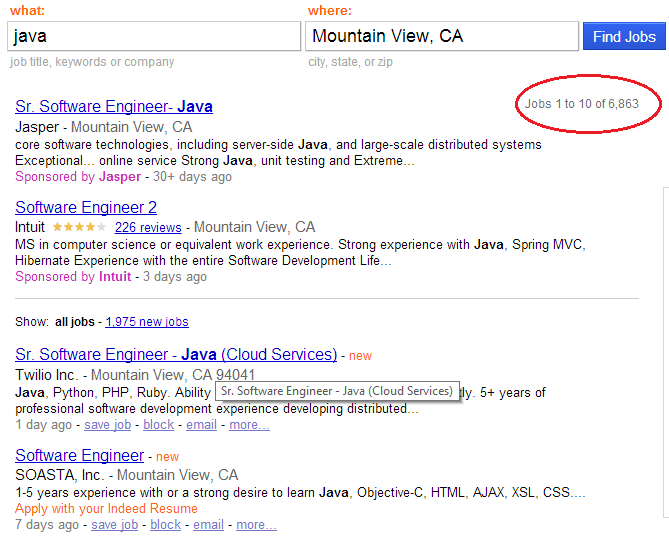
\includegraphics[scale=0.6]{images/indeed1.png}
  \caption{Search result of Indeed.com}
  \label{fig:Indeed}
\end{figure}

The reason for such a result is because current job searching web sites use the same information retrieval technology like ``Inverted index'' \cite{zobel2006inverted} as the common search engines, which just use keywords to map all the stored documents. Modern search engines all have some ranking algorithms to sort the search result, like page rank \cite{page1999pagerank}, so the top results always be the most related ones. But such algorithms are unavailable to the job search systems, because the criteria  of how to rank the job searching result is very personalized. A great job opening for one job seeker maybe looks not good to the other, because the goodness of a job to a specular job seeker is heavily depend on his personal background, like his education or professional experience etc.

Since the people's r\'esum\'es contain the most important background information, we believe the content of the r\'esum\'e could be used to rank the job openings. We give an example of r\'esum\'es in Table~\ref{tab:resume}. In this thesis, we created a web system which uses the r\'esum\'es of job seekers to find the jobs that match their profiles best. The main idea is to calculate the similarity between the r\'esum\'e model and job models, which should be generated from r\'esum\'es and job descriptions. We want to transfer the job searching task from key word searching to candidate model matching. The matching result should be sorted by the matching score, higher matching score means a better matching. The matching algorithm does not only help job seekers to find the appropriate jobs, but also offers priority to them~\cite{gueutal2006brave}.  The job with higher matching score means the job is more appropriate to the job seeker, and if he applies to the job, the chance of getting the interview will be higher as well. Figure~\ref{fig:Matching} shows how this approach works.


\begin{figure}[htbp]
  \centering
  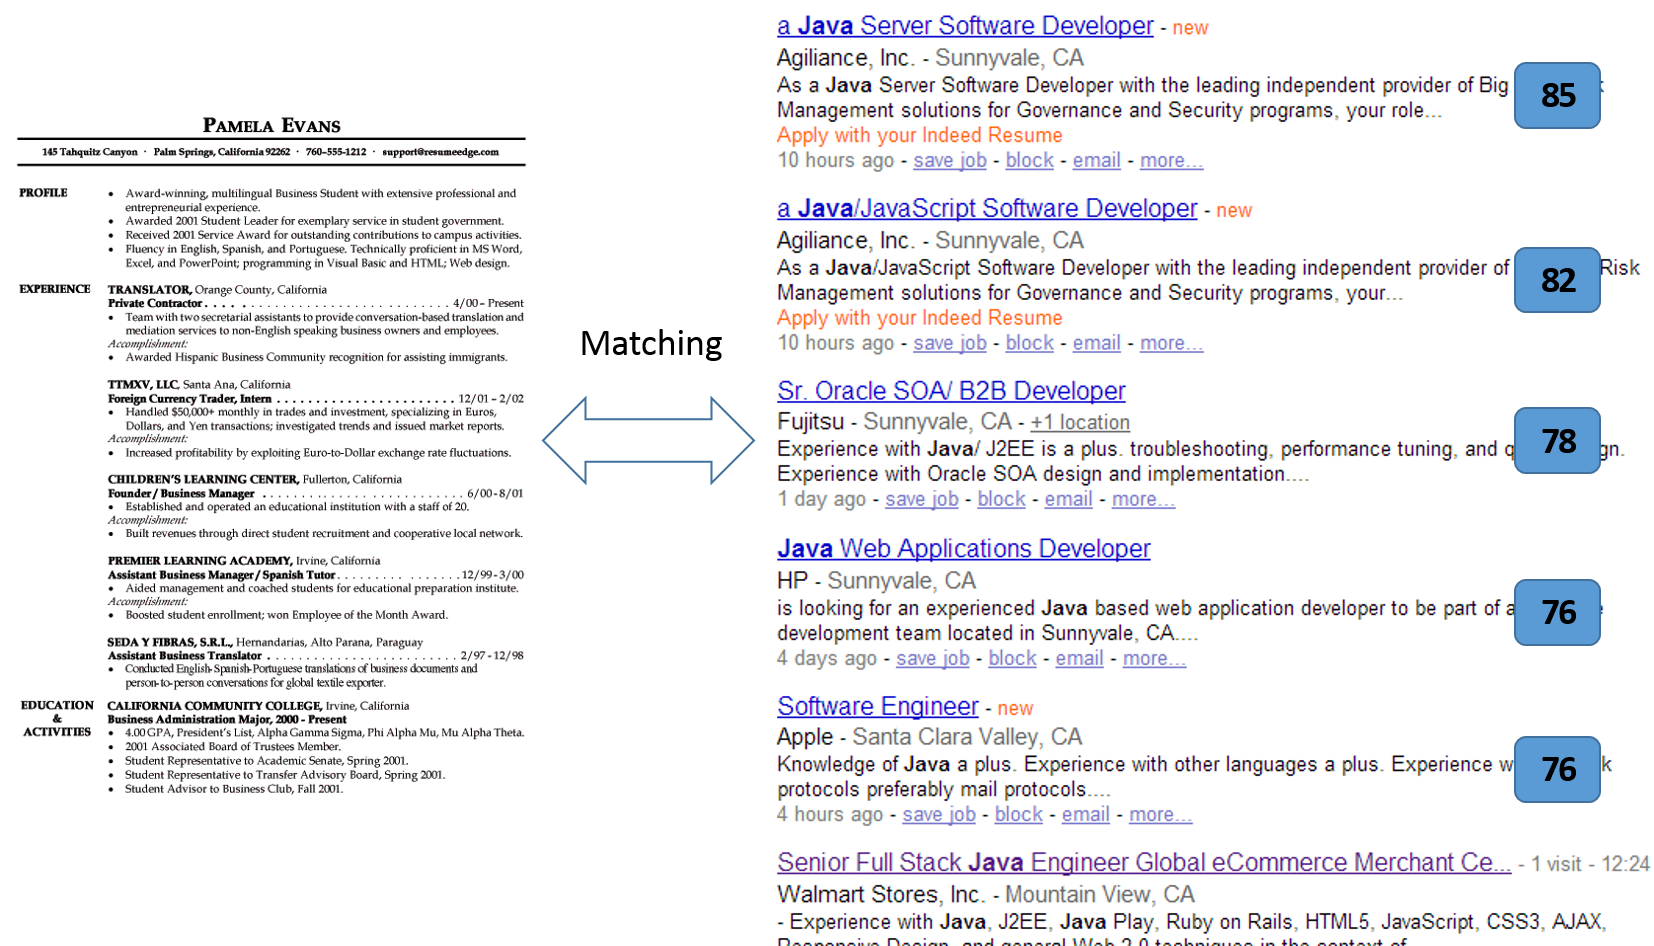
\includegraphics[scale=0.5]{images/matching.png}
  \caption{Matching the jobs with Resume}
  \label{fig:Matching}
\end{figure}


\begin{table}[!p]
 \small
\caption{R\'esum\'e Example} % title of Table
\centering % used for centering table
\begin{tabular}{    |  p{15cm} |  }
\hline
\begin{center}\normalsize{\textbf {Ryan Richman}}\\
\end{center}
\\
WORK EXPERIENCE\\
\\
\textbf{Web Developer}\\
Fabuso/Advanced Brain Technologies - Ogden, UT - February 2012 to Present \\
Created dynamic custom web applications for e-commerce and B2B clients. \\
Designed and edited audio-visual content for many different online applications. \\
Spearheaded migration of largest client's website from Joomla platform into Java code base. \\
Built dynamic event pages, document viewers, training course applications, shopping carts, and more. \\
Utilized advanced e-mail standards and best practices, SQL database queries, and Google Analytics.\\
\\
\textbf{IT Representative}\\
Advanced Brain Technologies - Ogden, UT - April 2011 to February 2012 \\
Provided internal software/hardware support for 20 employees both in-house and remote. \\
Designed using wireframes, tested, and debugged web pages. \\
Constructed dynamic projects and graphic designs in coordination with senior developers. \\
Created HTML-optimized emails for hundreds of campaigns. \\
Maintained and upgraded hardware for 20+ workstations company-wide. \\
\\
\textbf{Founder/Head Technician}\\
Teton Media Services, LLC - Ogden, UT - October 2008 to January 2011 \\
Created and developed websites for personal and small business customers \\
Sold high-speed cable and satellite internet access on the phone, online and in person. \\
Installed and serviced high-speed internet access hardware in residential and commercial properties. \\
Designed and implemented networking solutions for homes and businesses. \\
\\

\\
EDUCATION\\
\\
Computer Science \\
Weber State University - Ogden, UT 2010 to 2013 \\
\\
ADDITIONAL INFORMATION \\
\\
Technical Skills \\
Adept in the use of HTML, CSS, jQuery, Javascript, SQL, PHP, JSON, Windows, Windows Server, Mac, and Photoshop. \\

\\
\hline

\end{tabular}
\label{tab:resume} % is used to refer this table in the text
\end{table}


\section{Contribution}

We make the following contributions in this work:

\begin{enumerate}
    \item  We proposed a r\'esum\'e - job matching system.
    \item  We proposed a finite state transducer based matching tool to extract information from unstructured data source, which is a lightweight and flexible library, and can be extended in very easy ways.
    \item  We proposed a semi-automatic approach, which can collect technical terms from hr data sources, and by which we created a domain specific ontology for recruitment.
    \item  We proposed statistical-based ontology similarity measure, which can measure the similarities between technical terms .
\end{enumerate}

\section{Organization}
The subsequent chapters are organized as follows: we first describe what has been done in terms of prior work.  We introduce some basic conception of recommender systems, and how to apply recommender technologies into Job Recommender Systems. Some previous Job Recommender Systems will be introduced,  their advantages and limits will be discussed as well.  Two import problems of content-based Job Recommender Systems, Information Extraction and Similarity Calculation, will be fully explained.

Then we introduce our work, R\'esuMatcher, a the Personalized R\'esum\'e-Job Matching System. First, we give an overview of the system, which includes the architecture and the interfaces. Then we explained details of how we resolve the problems of information extraction and model similarity calculation. We propose a finite state transducer library which can match patterns in sentence, and extracts related information. Ontology plays an important role in this system. We will present how to construct the domain specific ontology for recruitment. We also give a brief review of different ontology similarity measures, and explain the statistical-based ontology similarity measure we used in this system.

Finally, we evaluate the accuracy of our information extraction approach. We used NDCG to evaluate the accuracy of statistical-based ontology similarity measure. To evaluate the performance of the system, we compared our algorithm to some classical information retrieval approaches by precision@k and NDCG. We created a data set of job descriptions as documents, and use r\'esum\'es as query to retrieval documents. The result shows the ranking performance is better than other information retrieval approaches.

\chapter{BACKGROUND}

Some scholars found that current Boolean search and filtering techniques cannot satisfy the complexity of candidate-job matching requirement~\cite{malinowski2006matching}. They hope the system could understand the job requirement, determine which requirements are mandatory and which are optional but preferable. So they moved to use recommender systems technique to address the problem of information overflow. Recommender systems are broadly accepted in
various areas to suggest products, services, and information items to latent customers.


\section{Recommender System}

Job searching is not a new topic in information retrieval, which has been the focus of some commercial job finding web sites and research papers. Usually scholars called them Job Recommender Systems (JRS), because most of them used technologies from recommender systems. Wei et al. classified Recommender Systems into four categories~\cite{wei2007survey}: Collaborative Filtering, Content-based filtering, Knowledge-based and Hybrid approaches. Some of these techniques had been applied into JRS; Zheng et al.~\cite{siting2012job} and AlOtaibi et al.~\cite{al2012survey} summarized the categories of existing online recruiting platforms and listed the advantages and disadvantages of technical approaches in different JRSs. The categories include:

\begin{enumerate}
    \item Content-based Recommendation (CBR). The principle of a content-based recommendation is to suggest items that have similar content information to the corresponding users, like Prospect \cite{singh2010prospect}.

    \item Collaborative Filtering Recommendation (CFR). Collaborative filtering recommendation, which finds  similar  users  who have  the same taste with the target user and recommends items based on what the similar users, like CASPER~\cite{rafter2000personalised}.

    \item Knowledge-based Recommendation (KBR). In the knowledge-based recommendation, rules and patterns obtained from the functional knowledge of how a specific item  meets the requirement of a particular user, are used for recommending items, like  Proactive~\cite{lee2007fighting}.

    \item Hybrid recommender systems combine two or more recommendation techniques to gain better performance, and overcome the drawbacks of any individual one. Usually, collaborative filtering is combined with some other technique in an attempt to avoid the ramp-up problem.

\end{enumerate}

\section{Job Recommender Systems}

Rafter et al. began to use ACF (Automated Collaborative Filtering) in their Job Recommender System, ``CASPER''  \cite{rafter2000personalised}. In the system user profiles are gotten from server logs, that included: revisit data, read time data, and activity data. All these factors were viewed as measure of relevance among users. The system recommend jobs in two steps. First the system find a set of user related to the target user, second the jobs that related users liked will be recommend to the target user. The system use cluster-based Collaborative Filtering strategy. The similarity between users are based on how many jobs they both reviewed, or applied.

The CASPER also allows user search jobs by a query which is a combination of some fields, like location, salary, and skill etc. The system use such query to find jobs, and the returned jobs will be ranked with above collaborative filtering algorithm.
In their paper, they didn't give a detail description on how to detect the related fields they need and how to the transfer semi-structured job description to structured one.

The shortages of Collaborative Filtering: First since the searching the number of searching result is huge, and the result is sorted randomly, even two very similar users may review different jobs,  or say the probability of two similar users reviewing the same job is low. The authors also noticed the such sparseness problem in users profile, so they try to user cluster-based solution to resolve this problem. Second because recommended jobs are from others users searching result, since the current quality of current searching result is low, so the quality of recommendation cannot be high.

F{\"a}rber et al \cite{farber2003automated}. presented a recommender system built on a hybrid approach. The system integrated two methods, content-based filtering and collaborative filtering, and tried to overcome the problem of rating data sparsity by leveraging synergies of a combined model, et. the  latent aspect model. The data they used were synthetic resume. The model they are shown in Figure~\ref{fig:la}.


\begin{figure}[htbp]
  \centering
  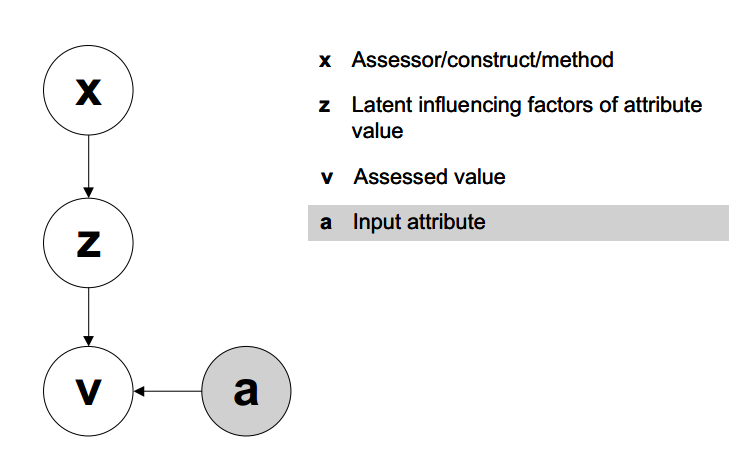
\includegraphics[scale=0.4]{images/la.png}
  \caption{Latent Aspect Model}
  \label{fig:la}
\end{figure}

In Malinowski et al. \cite{malinowski2006matching}, they classified the job recommender systems into two categories,  CV-recommender, which recommends CVs to recruiter, and the job-recommender, which recommends jobs to job seekers. The system collect the users' profile data by asking input their profiles to the web form based interface field by field. The input data collected are:

\begin{enumerate}
    \item  Demographic data (e.g. date of birth, contact information)

    \item  Educational data (e.g. school courses, grades, university, type of degree, intermediate and final university examinations, postgraduate studies)

    \item  Job experience (e.g. name of the company, type of employment, industry group, occupational field)
    \item  Language skills (e.g. language, level of knowledge)
    \item  IT skills (e.g. type of skill, level of knowledge)
    \item  Awards, scholarships, publications, others

\end{enumerate}
The system also asked the users upload their resumes, but that's for facilitating the human judgment.

From the paper we know, the model latent aspect model is a statistical model, which need to be trained before be applied into recommendation. But training need user to label to data, since current quality of result of job searching is poor, it will take a lot of time for user to train model.

Ioannis et al. used a machine learned prediction model to recommend new jobs to job seekers~\cite{paparrizos2011machine}.  The features used by the prediction model includes:

\begin{table}[ht]
\caption{Resume and Job Description} % title of Table
\centering % used for centering table
\begin{tabular}{ l l r }
 \hline
 Feature type &  Feature  &  Range   \\ \hline
              &  company title   & String  \\
Institution   &  industry        & String  \\
              &  company type    & \{public, private\} \\
              &  number of employees &    Num \\
 \hline
              &  number of jobs         & Num  \\
              &  position title         & String  \\
  employee    &  best position title    & String \\
              &  years of experience    &    Num \\
              &  number of universities &    Num \\
              &  education degree       & String \\
 \hline
\end{tabular}
\label{tab:predictionmodel} % is used to refer this table in the text
\end{table}


\section{Information Extraction in Job Recommender System}

Some big IT companies had meet a similar problem of information overflow. Any position they published, will receive a lot applications. The recruiter need to screen the all the applications, but this task is also tedious and time consuming, highly cumbersome and inefficient. so these company tried to build systems to help screen the position candidates.

Amit et al. in IBM presented a system, ``PROSPECT''~\cite{singh2010prospect}, to aid    shortlisting of candidates for jobs. The system uses a resume miner to extract the information from resumes, which use a CRF model to segment and label the resumes. The CRF model used three kinds of features, they are: Lexicon, Visual, Named Entity, Text, and Conjunction. The paper compared some algorithms to ranked the candidates applicants, such methods include: Okapi BM25, KL, Lucene Scoring, and Lucene Scoring + SkillBoost.

HP also built a system to solve the similar problem, which is introduced in Gonzalez et al.'s paper~\cite{gonzalez2012adaptive}. The system also pays a lot of attention to information extraction. The IE architecture they use is shown in Figure~\ref{fig:hpie}.


\begin{figure}[htbp]
  \centering
  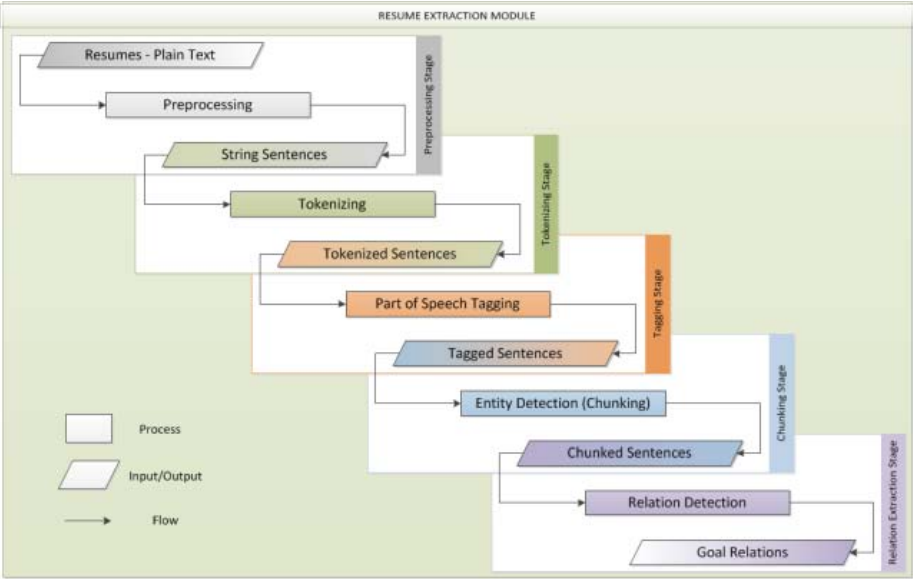
\includegraphics[scale=0.5]{images/hpie.png}
  \caption{IE Framework}
  \label{fig:hpie}
\end{figure}

The dictionaries which were used to tag entities should be updated often since there always new terms appears. So an adaptive learning module is used to achieve two objectives: use semantic data to enhance the information extraction and to discover new terms.

A domain-oriented ontology is used to represent knowledge, inference rules are defined based on the ontology knowledge base. When a detected term found, the system will search in external knowledge base, like DBpedia etc. The resume also be classified to different categories like ``Web Technology'' and ``No Web Technology'' by naive Bayes classifier. The company could allocate appropriate employees to required positions.

\begin{table}[ht]
\caption{Comparison of Job Recommender Systems } % title of Table
\centering % used for centering table
\begin{tabular}{ | c |  p{6cm} | p{6cm} | } % centered columns (4 columns)

\hline  %inserts double horizontal lines
 System & Approach  & User Information  \\ [0.5ex] % inserts table
%heading
\hline % inserts single horizontal line
 &
    \begin{singlespace}
       \textbullet~Declarative  \par
       \textbullet~Easy to comprehend  \par
       \textbullet~Easy to maintain\par
       \textbullet~Easy to incorporate domain knowledge\par
       \textbullet~Easy to trace and fix the cause of errors  \par
    \end{singlespace}
    &  \begin{singlespace}
      \textbullet~Heuristic \par
       \textbullet~Requires tedious manual labor \par
       \end{singlespace}   \\
\hline
ML-based &
    \begin{singlespace}
       \textbullet~Trainable  \par
       \textbullet~Adaptable \par
       \textbullet~Reduces manual effort \par
    \end{singlespace}
    &  \begin{singlespace}
      \textbullet~Requires labeled data \par
       \textbullet~Requires retraining  for domain adaptation \par
        \textbullet~Requires ML expertise  to use or maintain \par
       \textbullet~Opaque  \par
       \end{singlespace}  \\
\hline %inserts single line
\end{tabular}
\label{tab:jrcom} % is used to refer this table in the text
\end{table}

Yu et al.~\cite{yu2005resume} used a cascaded information extraction (IE) framework to get the detailed information from the job seeker��s resume. In the first stage, the Hidden Markov Modeling (HMM) model is used to segment the resume into consecutive blocks. Based on the result, a SVM model is used to obtain the detailed information in the certain block, the information include: name, address, education etc.

Celik Duygua and Elci Atilla proposed a Ontology-based R��sum�� Parser (ORP) ~\cite{ccelik2013ontology}, which uses ontology to assistant the information extraction process. The system process the resume in following steps: convert the resume files into plain text, separate the text into  some segments, use Ontology Knowledge Base to find the concepts in the sentences, normalize all the terms, at last the system will classify the sentences to get the wanted terms.

\section{Matching Algorithms in Job Recommender Systems}

Lu et al.~\cite{lu2013recommender} used latent Semantic Analysis(LSA) to calculate similarities between jobs and candidates, but they only selected two factors ``interest'' and ``education''  to compare candidates. Xing et al.~\cite{yi2007matching} used Structured Relevance Models (SRM) to  match resumes and jobs.

Drigas* et al.\cite{drigas2004expert}  presented a expert system to match jobs and job seekers, and recommend unemployed to the positions. The expert system used Neuro-Fuzzy rule to evaluate the matching between user profile and job opening. The system use a relation matrix to represent the fuzzy relation between these specialities. The system need the training data to train that Neuro-fuzzy network. Both resume data and job opening data were manually input into the system.

Daramola et al.\cite{daramola2010fuzzy}  also proposed a fuzzy logic based expert system(FES) tool for online personnel recruitment. In the paper, the authors assumed that the information already be collected. The system use a fuzzy distance metric to rank candidates' profile in the order of their eligibility for the job. The fuzzy hamming distance is given as:
$$ \delta \left ( O,R \right )=\sum_{i=1}^{n}\left | \mu_O(x_i) - \mu_R(x_i)  \right | $$

Yao et al.~\cite{lu2013recommender} also presented a hybrid recommender system which integrated content-based and interaction-based relation. In content-based part, relations between job-job, job-job seeker, and job seeker - job seeker could be identified by their similarity of profiles. There two approaches are used to calculate the similarities: For the structured data, like age gender  etc., the weight sum values will be returned, for the unstructured data like similarity between job and user profile the Latent Semantic Analysis will be used.




\chapter{PROBLEM}

The basic problem in this thesis is how to found appropriate job descriptions by user's resume. If we take the resume as query, the job descriptions as documents, we need build a information retrieval model to get the most relevance documents.  The JobFinder will parse the job descriptions to the job models, and store them in the database. When a user searches the jobs by their resume in the system, the system will compare the similarity values between the resume and the job models, and return the job sorted by their similarity value.

The core idea of our algorithm is calculate similarity between resume model and job model.
We give a formal definition of our problem. All of the notations will be used frequently throughout the thesis.

We use $r$ denote the user's resume model, $r$ has some features $r_i$ like academic degree, their major, their skill set and so on. The symbol $J$ is the set of job models stored in the database, $j$ is a job model in the se $J$. The similarity function $sim(r, j)$ gives the similarity value between resume $r$ and job $j$. The return list of search function $search(r,J)$ will calculate all the similarity value in the database, and the result of the function will be the job description list ranked their similarity value. The equation of how to calculate similarity value is given below:

$$ sim(r, j) = \sum_{i=1}^{n} simfun_i(r_i,j_i) \times w_i $$

The value of $sim(r, j)$ is summation of similarity value of different fields times their corresponding weight, which means different fields like major and skills,  may have different approaches to calculate their similarity value. We will describe the similarity functions of individual fields in later parts.

\chapter{System Overview}

\section{System Overview}
The system will use rule based information extraction technique to parse job descriptions and resumes, and get information such as skill, specialties and background. These information will be used to create the model of job openings and job seekers. Ontology will be used to construct the knowledge base, which will include the taxonomy, to support resume-job matching.

The models of resume will include job seekers' specialties, working experience and education background, all the fields will be extracted from their resumes. The job models will be extracted from job descriptions, and have the same information fields as the resume models.  When a job seeker searches the jobs by his resume, the system will calculate the similarity between the candidate model and the job models, give every job model a similarity score.

\section{System Architecture}

Figure ~\ref{fig:Pipeline} shows the architecture of the whole system, which include such modules:

\begin{enumerate}
    \item The web scrawler could search and download all new IT job opening web pages  from indeed.com everyday.
    \item Job parser could parse the job opening web page, extract the information and create the job model.
    \item Resume Parser is much like the Job parser, it will parse the resume and create the candidate model.
    \item All the job models will be stored in the Job Description database.
    \item When user make a query request, the ontology matcher will calculate the matching score of each job, return the jobs ranked by their scores.
\end{enumerate}

\begin{figure}[htbp]
  \centering
  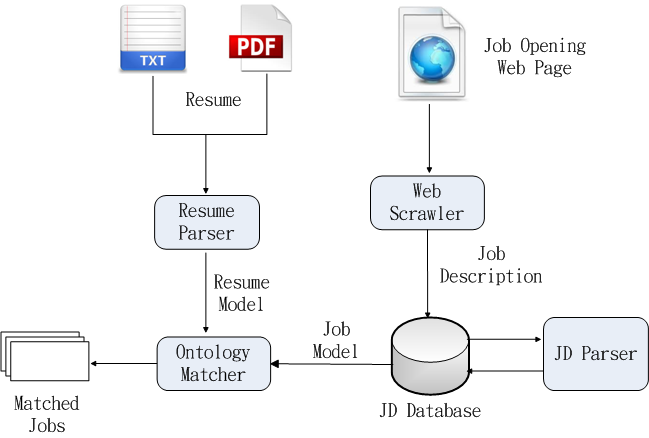
\includegraphics[scale=0.5]{images/arch.png}
  \caption{System Architecture}
  \label{fig:arch}
\end{figure}

\section{System Implementation}

We describe some implementation details here. The whole system was implemented in Python, and used some third party libraries and frameworks. For the web module we used Flask, a lightweight web framework. We used Rdflib as the OWL file parser, PLY(Python Lex-Yacc) as the token regular expression compiler, whoosh as the unversed index builder and Beautiful Soup as the HTML parser.  All the jobs get by the web crawler are stored in the MongoDB NoSQL database.  For the natural language processing part, we used NLTK and pattern to extract the sentences and tokenized the sentences.

\section{System Interface}

The system provide some interface to end users. The most important interface include review all the jobs in the database, search the jobs by keyword Figure~\ref{fig:joblist},  upload user resume ~\ref{fig:upload_resume}, the resume matching result~\ref{fig:match_resume} and search the jobs with both keyword and resume~\ref{fig:keyword_resume}.

\begin{figure}[htbp]
  \centering
  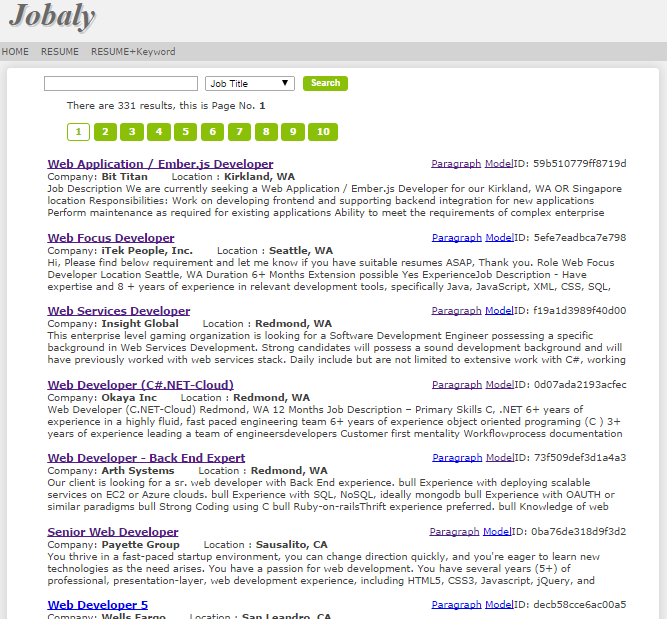
\includegraphics[scale=0.5]{images/joblist.png}
  \caption{Job Description List}
  \label{fig:joblist}
\end{figure}


\begin{figure}[htbp]
  \centering
  
\includegraphics[scale=0.5]{images/upload_resume.png}
  \caption{Upload Resume}
  \label{fig:upload_resume}
\end{figure}

\begin{figure}[htbp]
  \centering
  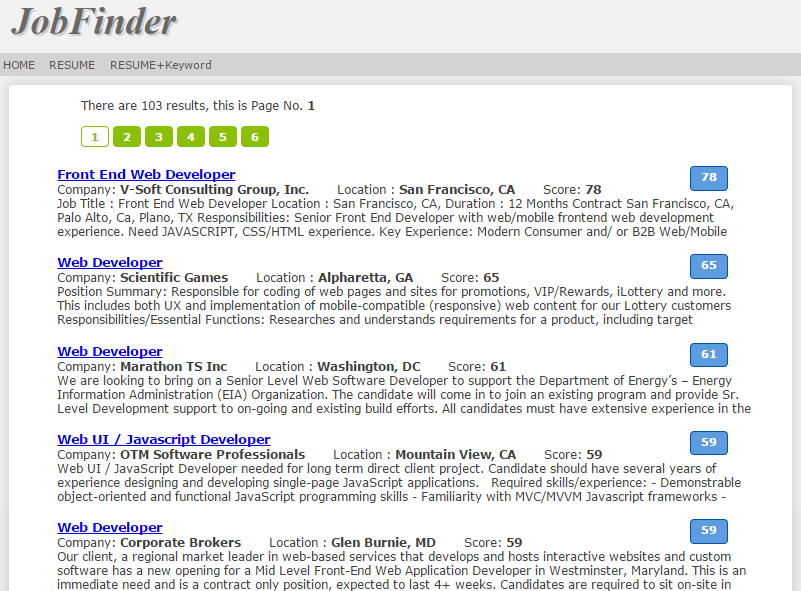
\includegraphics[scale=0.5]{images/match_resume.png}
  \caption{Resume Job matching }
  \label{fig:match_resume}
\end{figure}

\begin{figure}[htbp]
  \centering
  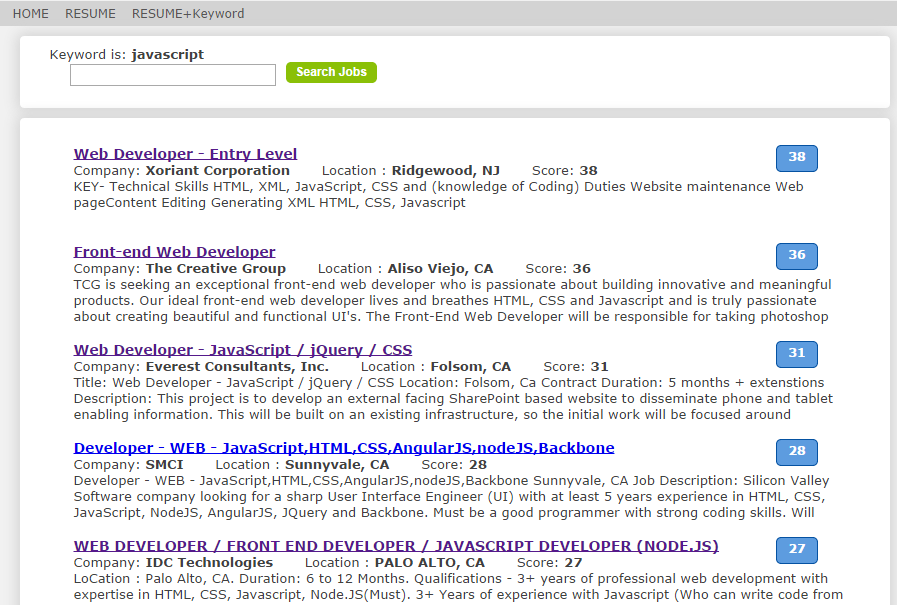
\includegraphics[scale=0.5]{images/keyword_resume.png}
  \caption{Combine the Keyword and Resume Matching}
  \label{fig:keyword_resume}
\end{figure}







\chapter{Information Extraction}

To calculate the similarity between a job and a resume, JobFinder system need the models of them, which are  structured data. To get the structured data, some JRSs ask the job seekers input their profiles in forms field by field, and the recruiter input their job description in the same way as well. However, as we discussed in chapter 2, the users are reluctant to take the tedious process ~\cite{singh2010prospect}. Job seekers prefer upload their resumes directly, and recruiters prefer to post the whole job description to web sites. In this chapter we will explain how the Information Extraction module of the system extracts information from these unstructured data source.

Information Extraction is the task of automatically extracting structured information such as entities, relationships between entities, and attributes describing entities from unstructured sources. ~\cite{sarawagi2008information}.  The IE framework will be introduced below by example of processing the job descriptions, and the FST library, which is used as pattern matching tools, will be introduced as well.

\section{Text Processing Stages}

The IE framework uses six stages in order to extract the information from job descriptions: HTML parsing, segmenting, preprocessing, tokenizing, labeling and pattern matching, which is show in Figure~\ref{fig:Pipeline}.

In Nature Language Processing, especially in Information Extraction, pipeline is a well adopted architecture~\cite{sarawagi2008information}. The pipeline to process the job descriptions in the system has eight stages, which is shown in Figure~\ref{fig:Pipeline}:

1) The HTML parser will parse the web pages that contain job descriptions, which are obtained from web crawler. The parser uses HTML tag template to extract attributes of the jobs, like job title, location, company name and content. A job will be saved as a record with these attributes in the database. In the record, the field content contains the text part of the job description, which will be the processed in later stages.

2) In the segmenting stage, the content field of the job description is be separated into paragraphs according HTML tags. Then paragraphs are separated into sentences by either HTML tags or punctuations, and after this step, all HTML tags will be removed.

3) The web pages of job description are created in different character sets, e.g. UTF8 and ISO 8859-1, and always contain some unreadable characters. In the prepossessing stage, characters in the sentences are converted to the ASCII characters, unreadable characters will be deleted, some punctuations will be replaced by spaces e.g. / and -.

4) In the tokenizing stage, the sentences will be tokenized into arrays of tokens by NLTK \cite{bird2006nltk}.

5) In the labeling stage, the sentences will be given two layers of labels by a dictionary matching approach. The labels in the first layer are the semantic value of the text, and the labels in the second layer are the ontology hypernym of the first layers.

6) In the pattern matching stage, the FST library is used to matching the labels of the labeled sentences.  If a layered sentence match any pre-defined pattern, the information will be extracted and added to the job model. After every sentence of a job description has be processed, a job model will be created and saved in the database.

\begin{figure}[htbp]
  \centering
  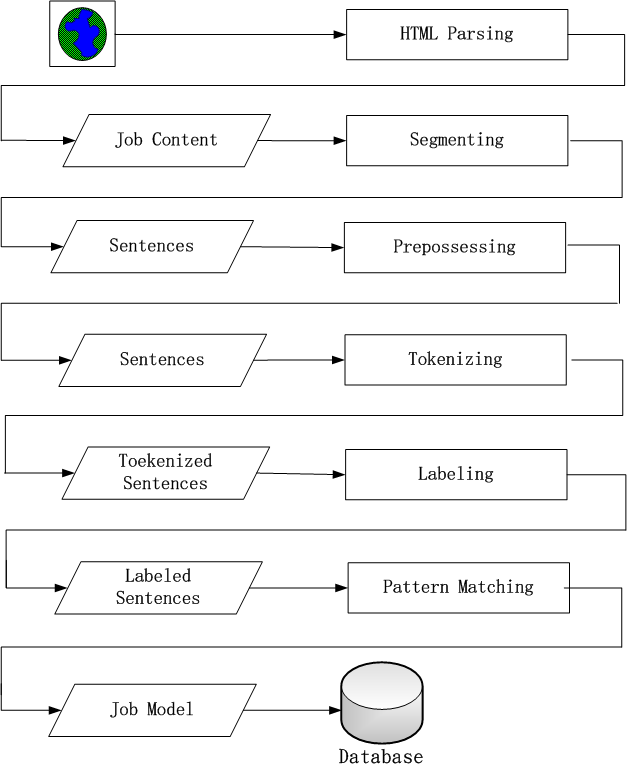
\includegraphics[scale=0.4]{images/pipeline2.png}
  \caption{Job Description Process Pipeline}
  \label{fig:Pipeline}
\end{figure}

\section{Semantic Labeling}

In this section, we will introduce why and how we add two layers of label to the tokenized sentences. In natural language, one concept always have some different expressions. For example, the simple concept bachelor's degree,  has several expressions in job descriptions, e.g. B.S., BA/BS, 4 years degree, and so on. The Table \ref{tab:multispelling} shows the words that if followed with word ``degree'' have the semantic value of ``bachelor's degree''.

\begin{table}[ht]
\caption{All words have meaning bachelors } % title of Table
\centering % used for centering table
\begin{tabular}{  | p{15cm} |  }
 \hline
 "Baccalaureate","bachelors", "bachelor" ,"B.S.", "B.S","BS","BA","BA/BS", "BABS", "BSBA", "B.A." ,"4-year","4-year", "4 year", "four year","college","Undergraduate" , "University" \\
  \hline
\end{tabular}
\label{tab:multispelling} % is used to refer this table in the text\section{Pipeline of Information Extraction}
\end{table}

The regular expression over tokens will transfer a patten to a Finite-State Transducer(FST), and every token of the pattern will be transferred to a state of FST. If we use all the expressions of a semantic value to create a pattern, the pattern will be very large, and there are too many states in the FST. For example, if we use some words in Table~\ref{tab:multispelling} to create the pattern of semantic value ``bachelor's degree'', the pattern will like below:

$$ (~Baccalaureate~\mid~bachelors~\mid~bachelor~~\mid~B.S~\mid~BS~\mid~BA~)~~degree $$

If all words in Table~\ref{tab:multispelling} are added to the pattern, the FST will have too many states, and the matching process will be very slow because of the problem of combinatorial explosion.

To resolve this problem, we proposed an approach to use the patterns match the labels of the tokens, not the the original text. Because in the system, we don't care what the words the sentences really use, but want to extract the semantic value of the tokens which match the pattern. The details of the approach is described below:

At first, we created two dictionaries, which are used to labeling the tokens. In the first dictionary, the keys are the tokens, like words in Table~\ref{tab:multispelling}, and the values are the symbols for semantic values, like ``BS-LEVEL'' for ``bachelor's degree'', or ``MS-LEVEL'' for ``master's degree''. In the second dictionary, the keys are semantic values, which are the values of first dictionary. The values of the the second dictionary are the ontology hypernym of their keys, like keys ``BS-LEVEL'' and  ``MS-LEVEL'' both have value ``DE-LEVEL'', which means that bachelor's degree and master's degree are both one kind of degree level.

With the two dictionaries, we can labeling the tokens with two layers. In the first layer, we labeled the tokens with its semantic values, which are the values that we want to extract from the sentence. In the second layer, the labels, which will be matched with patterns, are the ontology hypernyms of the labels in first layer. Table~\ref{tab:labeldsent} shows how the sentence ``Bachelors  degree  in computer science or information systems. '' is labeled.

\begin{table}[ht]
\caption{Labeled sentence } % title of Table
\centering % used for centering table
\begin{tabular}{  | c | c | c | c | c |c | c |c | c | c |  }
 \hline
 layer 2 & DE-LEVEL   & DEGREE & IN & MAJOR            & OR & MAJOR  &.  \\
 \hline
 layer 1 &  BS-LEVEL   & DEGREE & IN & MAJOR-CS         & OR & MAJOR-INFO & .      \\
 \hline
   words & bachelors   & degree & in & computer science & or & information systems & .     \\
  \hline
\end{tabular}
\label{tab:labeldsent} % is used to refer this table in the text\section{Pipeline of Information Extraction}
\end{table}

The pattern ``DE-LEVEL DEGREE  IN   MAJOR  OR  MAJOR ''  matches the sentence above, and the output of the sentence is ``BS-LEVEL'' for bachelor's degree. In the system most patterns match the labels in second layer. With this approach, the states in the pattern will be minimized.

\section{Pattern Matching}

As we explained in last section, we used some patterns over labels in second layer to match the sentences. Some patterns used to match degree phases are in Table ~\ref{tab:patterns}. The patterns looks like regular expression, but they use tokens as the basic units.

\begin{table}[ht]
\small
\caption{Patterns match degree} % title of Table
\centering % used for centering table
\begin{tabular}{  | l  |  }
 \hline
 DE\_LEVEL,  DE\_LEVEL, OR  DE\_LEVEL DEGREE   \\
 DE\_LEVEL DEGREE ( IN  $\vert$  OF ) DT MAJOR   \\
 MAJOR\_DEGREE  ,  MAJOR\_DEGREE OR MAJOR \\
 DE\_LEVEL (, DE\_LEVEL)* (OR DE\_LEVEL)? BE? PERFER\_VBD   \\
 \hline
\end{tabular}
\label{tab:patterns} % is used to refer this table in the text\section{Pipeline of Information Extraction}
\end{table}

To matching the labels in sentences, we proposed a library that support matching pattern over tokens. The difference between this library and traditional regular expression is that the basic unit to be matched is token, not character. In the library, a matcher could be a token to be matched, and also could be composition of other matchers. The library supports syntax used in traditional regular expression over string, we list the syntax that the library supports in Table~\ref{tab:matchers}. The first column is the names of the matchers, the second column is the explanation of the function of the matchers, and third column is the their counter part syntaxes of traditional regular expression. The RegexMatcher in library has a regular expression that matches any token matching the regular expression. We give examples of the syntax of these matchers in Table \ref{tab:matchers_example}.

\begin{table}[ht]
\caption{Matcher Class } % title of Table
\centering % used for centering table
\begin{tabular}{  | l | l | l |  }
 \hline
 Matcher Name        &  Function                                 & Counter Part of regex    \\
 \hline
 UnitMatcher       &  token is matches the it                  & character  in regex       \\
 \hline
 SequenceMatcher   &  A list of Matcher                        & sequence of characters       \\
  \hline
 QuestionMatcher   &  One or more of the preceding token       & ?       \\
  \hline
 StarMatcher       &  Zero or more of the preceding token      & *       \\
  \hline
 PlusMatcher       &  Zero or one of the preceding token       & +       \\
  \hline
 DotMatcher        &  Any token                                & .      \\
  \hline
 RegexMatcher      &  Any token matches the regular expression               &        \\
  \hline
\end{tabular}
\label{tab:matchers} % is used to refer this table in the text\section{Pipeline of Information Extraction}
\end{table}



\begin{table}[ht]
\caption{Matcher Class } % title of Table
\centering % used for centering table
\begin{tabular}{  | l |  l |  }
 \hline
 Matcher Name          & Example    \\
 \hline
 UnitMatcher         & DEGREE       \\
 \hline
 SequenceMatcher     & DE-LEVEL DEGREE       \\
  \hline
 QuestionMatcher     & DE-LEVEL (OR DE-LEVEL)?  DEGREE       \\
  \hline
 StarMatcher         & DE-LEVEL (, DE-LEVEL)*  DEGREE       \\
  \hline
 PlusMatcher         & DEGREE IN MAJOR +      \\
  \hline
 DotMatcher          & HAS . DEGREE      \\
  \hline
 RegexMatcher        & r``d-d'' years  \\
  \hline

\end{tabular}
\label{tab:matchers_example} % is used to refer this table in the text\section{Pipeline of Information Extraction}
\end{table}


\section{Regular Expression Over Tokens}

In last section we generally introduced how we use the library of regular expression over tokens to match the sentences. In this section we will introduce more details of this library, like its advantages and implementation details.

\subsection{Finite-State Transducer}
Finite-State Transducer\ref{roche1997finite} is used as a tool to match patterns and extract information for more than 20 years. This approach have been demonstrated very effective in extracting information from text like CIRCUS~\cite{lehnert1991university} and FASTUS~\cite{hobbs199713}.  In the widely used NLP toolkit GATE~\cite{cunningham2002framework}, the semantic tagger JAPE (Java Annotations Pattern Engine) could describe patterns that are used to match and annotate tokens. JAPE adopts a version of CPSL (Common Pattern  Specification Language)~\cite{appelt1998common}, which provides FST over annotations. Chang et al. presented cascaded regular expressions over tokens~\cite{chang2014tokensregex}, which proposed a cascaded pattern matching tool over token sequences.

After studying these tools, we found most of them are powerful, complex, but not very flexible. One reason is that developers need to learn some DSLs like CPSL, and the other is  integrating the pattern matching tool into the system need extra efforts. So here we proposed a more flexible and lightweight FST framework, which can do regular expression matching over labeled tokens. We give the definition of Finite-State Transducer here. A Finite-State Transducer is a 6-tuple $(\Sigma_1, \Sigma_2, Q, i, F, E)$ where:
\begin{itemize}
  \item $\Sigma_1$ is a finite alphabet, called the input alphabet.
  \item $\Sigma_2$ is a finite alphabet, called the output alphabet.
  \item Q is a finite set of states.
  \item $i \in Q$ is the initial state.
  \item $F \subset Q$ is the set of final states.
  \item $E \subset  Q  \times \Sigma_1^* \times \Sigma_2^* \times Q$ is the set of edges.
\end{itemize}


For example, the FST $T_{d3} = \left(     \{ 0, 1 \} ,  \{ 0, 1 \} , \{ 0, 1 , 2 \} ,  E_{d3} \right ) $ where $E_{d3} = $ \{ ( 0, 0, 0, 0 ),   ( 0, 1, 0, 1 ), ( 1, 0, 0, 2 ), ( 1, 1, 1, 0 ), ( 2, 1, 1, 2 ), ( 2, 0, 1, 1 ) \}  is shown in Figure~\ref{fig:fst}.


\begin{figure}[htbp]
  \centering
  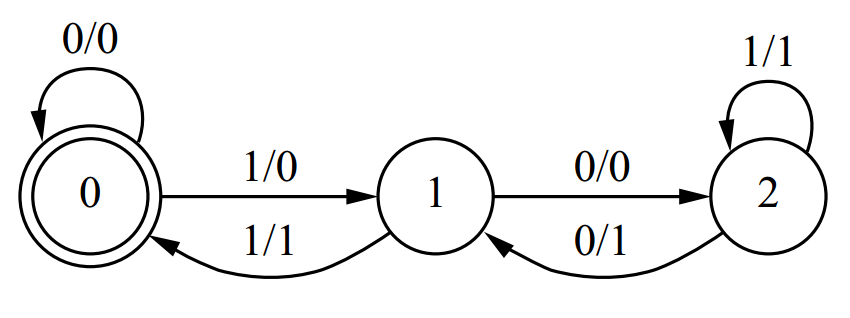
\includegraphics[scale=0.5]{images/fst.png}
  \caption{Zero or one NFA}
  \label{fig:fst}
\end{figure}


\subsection{Flexibility of the library}
The framework supports three styles to create patterns, which gives developers great flexibility. The most common style is defining pattern expression in a string, which is much like traditional regular expression. We give an example as follows:

\begin{framed}
\small
\begin{lstlisting}[language=Python]
seqMatcher =parser.parse("aaa | bbb ccc? * ddd")
\end{lstlisting}
\end{framed}

The seconde style is using algebra operator to connect matchers, as follows:
\begin{framed}
\small
\begin{lstlisting}[language=Python]
Pattern: " aaa (bbb | cccc)"
seqMatcher =  TokenMatcher("aaa") +
    TokenMatcher("bbb") | TokenMatcher("ccc")

\end{lstlisting}
\end{framed}

We also could create complex matcher in programming style, which is like we creating and using some objects when programming, as follows:

\begin{framed}
\small
\begin{lstlisting}[language=Python]
Pattern: " ( aaa | bbb ) cccc "
matcher1 = TokenMatcher("aaa")
matcher2 = TokenMatcher("bbb")
matcher3 = TokenMatcher("ccc")
matcher4 = AlternateMatcher([matcher1,matcher2])
seqMatcher = SeqMatcher([matcher3,matcher4])
\end{lstlisting}
\end{framed}


After labeling, the sentence become a sequence of arrays, each array includes the original token and its labels in the other two layers. The flexibility of the tool also comes from that developers could determine which layer of the array should be matched, the original text or labels in the first or second layer.  Developers can assign lambda expressions to the matcher's catching function, which defines how to get the matching input,  and out function, which defines what should be outputed. For example, to match the labeled sentence, we set the lambda expression for catching function to ``lambda x:x[2]'', and the out function to ``lambda x:x[1]'', which make the matcher match the label in second layer, and output the the value of semantic value in the first layer.

\section{Implementation of Finite Automata Matching Library }

To transfer a token regular expression to a Finite Automata Transducers(FST), we need two steps: The first is parsing the expression to a tree of matchers, the second is transfer the tree of matchers to the Finite Automata Transducers.

We use PLY(Python Lex-Yacc) as the grammar parser, which  is a pure-Python implementation of the popular compiler construction tools lex and yacc. We defined  grammars of token regular expression in the parser, which can parse the token regular expression to the tree structure.

We use the algorithm proposed by Thompson and Ken\cite{thompson1968programming} to construct the FST from the tree. The state for a regular expression is built up from partial Nondeterministic Finite Automaton (NFA)  for each subexpression, with a different construction for each operator. The partial NFAs have no matching states: instead they have one or more dangling arrows, pointing to nothing. The construction process will finish by connecting these arrows to a matching state.

The NFAs for matching single token is shown in Figure \ref{fig:nfa_single}.

\begin{figure}[htbp]
  \centering
  
\includegraphics[scale=1]{images/single_token.png}
  \caption{Single Token NFA}
  \label{fig:nfa_single}
\end{figure}

The NFA for the concatenation $e_1e_2$ connects the final arrow of the $e_1$ machine to the start of the $e_2$ machine, which is shown in Figure \ref{fig:nfa_cocat}.

\begin{figure}[htbp]
  \centering
  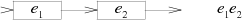
\includegraphics[scale=1]{images/concatenation_tokens.png}
  \caption{Concatenation NFA}
  \label{fig:nfa_cocat}
\end{figure}

The NFA for the alternation $e_1\mid e_2$ adds a new start state with a choice of either the $e_1$ machine or the $e_2$ machine, which is shown in Figure \ref{fig:nfa_alternation}.


\begin{figure}[htbp]
  \centering
  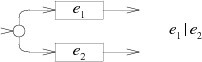
\includegraphics[scale=1]{images/alternation.png}
  \caption{Alternation NFA}
  \label{fig:nfa_alternation}
\end{figure}

The NFA for e? alternates the e machine with an empty path, which is shown in Figure \ref{fig:nfa_question}.


\begin{figure}[htbp]
  \centering
  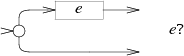
\includegraphics[scale=1]{images/question.png}
  \caption{Zero or one NFA}
  \label{fig:nfa_question}
\end{figure}

The NFA for e* uses the same alternation but loops a matching e machine back to the start, which is shown in Figure \ref{fig:nfa_star}.

\begin{figure}[htbp]
  \centering
  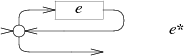
\includegraphics[scale=1]{images/star.png}
  \caption{Zero or more NFA}
  \label{fig:nfa_star}
\end{figure}

The NFA for e+ also creates a loop, but one that requires passing through e at least once, which is shown in Figure \ref{fig:nfa_plus}.

\begin{figure}[htbp]
  \centering
  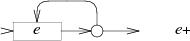
\includegraphics[scale=1]{images/plus.png}
  \caption{One or more NFA}
  \label{fig:nfa_plus}
\end{figure}



The expression like ``DL (, DL])*  (or DL)? DEGREE'' could be transferred to an FST in Figure ~\ref{fig:fst}.

\begin{figure}[htbp]
  \centering
  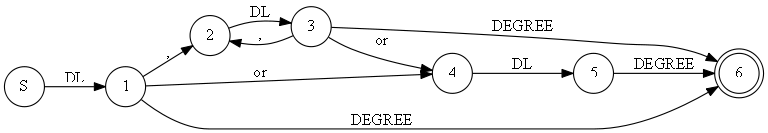
\includegraphics[scale=0.6]{images/test_tokenre2_6.png}
  \caption{Finite Automata Transducers}
  \label{fig:fst}
\end{figure}



\chapter{MODEL SIMILARITY}

In our system, the r\'esum\'e model and job model both have four fields: job title, major, academic degree and skills. The similarity value between a r\'esum\'e model and job model is the sum of the productions of similarity values of all the fields pairs and their weights. We will introduce how to calculate similarity value for each field in the chapter.

\section{Major and Academic Degree}

In the simplest case, if the majors in the r\'esum\'e model and job model are same, the similarity value is 1. If they are different, we can check whether the major in the r\'esum\'e model is in the list of related majors of the major in the job model. If it is, the similarity value is 0.5, otherwise the similarity value is 0. The equation is shown in below:

$$ MajorSim(r,j ) = \begin{Bmatrix}
1, & r_{major} = j_{major} \\
0.5, & r_{major} \in related( j_{major} ) \\
0, & otherwise
\end{Bmatrix} $$

There are five academic degree types in the system:  high school, associate, bachelor, master, and Ph.D. degree, which are mapped to the integer values form 1 to 5. If the degree value in the r\'esum\'e model is less than that in the job model, which means that the job seeker's education background cannot satisfy the requirement of the job, the similarity value in this case is 0. If the degree value in the r\'esum\'e model is equal to the job model, or no more than 2 bigger, the similarity value is 1. In some cases, the degree value in the r\'esum\'e model is greater than that of the job model, and the difference is greater than 2, which means the job seeker's degree is much higher than the requirement of the job. The situation is also a kind of relative matching, so the similarity value is given to 0.5. The equation is shown in below:

$$ DegreeSim(r,j ) = \begin{Bmatrix}
0,   & r_{degree} < j_{degree} \\
1,   & 0 < r_{degree} - j_{degree} \leqslant 2  \\
0.5, & r_{degree} - j_{degree} > 2
\end{Bmatrix} $$

\section{Job Title}

A job title can be parsed into some sub fields: job type, level, platform, programming language, and so on.  The value of job type includes: developer, manager, administrator and so on. The levels values are junior, senior, architect, and so on. The platforms include: web, mobile, cloud and so on. The similarity value between two titles is the sum of all the similarity values of these fields. If the job seeker has some working experience, there should be some job titles in their resume.  When calculating the similarity value between a r\'esum\'e model and a job model, the system calculates the similarity values of the title of job model to all the titles in the r\'esum\'e model, and return the maximum one.

We introduced how to calculate similarity values for three fields in r\'esum\'e and job models. In the next chapter, we will introduce how to use a domain specific ontology to calculate similarity value between the skills field of the two models.


\chapter{\uppercase{Ontology Construction and Similarity}}


\section{Semantic Similarity in JRSs}
After getting job models by the information extraction module, users can search for jobs in the system. In previous studies of JRSs, ontology is used as a knowledge base to store knowledge and rules, which could help compare the similarity between different concepts. Liu and Dew~\cite{liu2004using} used Resource Description Framework (RDF) to represent and store the expertise of experts, and they used a RDF-based expertise matcher to retrieve the experts whose expertise included the required concept.

Proactive~\cite{lee2007fighting} used two kinds of ontology, job category and company information. The system used an ontology checker to classify the job information, stored the domain knowledge and calculated the weight value in recommendations.

Fazel \cite{fazel2009semantic} used a hybrid approach to match job seekers and job postings, which takes advantage of the benefits of both logic-based and ontology-based matching. In his paper the description logics (DL) are used to represent the candidate and job opening, and the ontology is used to organize the skills in a taxonomy. The paper provides an equation to calculate the matching degree:
$$ sim\left(P ,j \right) = \sum x_{ij} \times u(ds_i) $$

where $x_{ji}$ is the Boolean variable indicating whether desire i is satisfied by applicant $A_{j}$ in the set of all qualified applications.

Kumaran et al.~\cite{kumaran2013towards} also used an ontology to calculate the similarity between the job criteria and candidates' r\'esum\'e in their system~\cite{kumaran2013towards}. The similarity equation they used is:
$$ M\left ( i_1, i_2 \right ) = \frac{\sum_{k=1}^{n} Sim\left (p_{k}^{i1},  p_{k}^{i2} \right ) * W_{k}^{i2}}{\sum_{k=1}^{n} W_{k}^{i2}}  $$
The similarity function $Sim(p_1, p_2)$ is defined as follows:
$$ Sim(p1, p2) = \begin{Bmatrix}
1, & if~similarity~of~p1~and~p2 \geqslant t\\
0, & otherwise
\end{Bmatrix} $$

\section{Ontology Construction}

Before calculating the similarity between concepts, we need to construct the ontology first. Semantic web has been a popular research topic in previous years, and at the same time thousands of domain ontologies have been created~\cite{ding2004swoogle}. A paradigmatic example is WordNet~\cite{fellbaum1998wordnet}, which is a general purpose thesaurus, and contains more than 100,000 general English concepts. ACM has created a poly-hierarchical ontology that can be utilized in semantic web applications~\cite{acm2012class}, but it is mostly used in academic areas. DBpedia~\cite{bizer2009dbpedia} provides structured information from Wikipedia and make this information available on the Web, but its coverage is huge, and most of them is not related to job finding. Currently, there is no domain specific technology ontology built for recruiting purpose.

The domain specific technology ontology for recruiting should include a lot of technical terms, like programming language, programming library, commercial products and so on. Furthermore, there are new techniques invented everyday, so new IT terms will appear continuously. Ding et al.~\cite{ding2002ontology} gave a survey of current ontology generation approaches such as manual, semi-automatic, and automatic. Some aspects of the approaches were discussed in the paper, like the source data, concept extraction methods, ontology representation, and construction tools. Inspired by this paper, we propose a semi-automatic approach to construct the IT skill ontology, which use a pattern matching approach to collect possible technical terms, and use DBpedia to verify the them.

From the observation, we found that sentences with skill requirements in job descriptions always list several skills in the sentence, which is shown in Table ~\ref{tab:skillrequirement}. Based on this character, we propose a bootstrap approach to collect IT terms in job descriptions.  First, we manually collect about fifty terms from job descriptions, and add them to the term list. Then we use our pattern match library to find the sentences that matching the pattern in Table \ref{tab:patterns} from a set of job descriptions. An example of a sentence which matches the pattern is shown in Table \ref{tab:termspattern}. We extract the tokens which match the star symbol from the sentences; these tokens have high probability to be technical terms. Then we could check the tokens in Dbpedia to see whether they are under the categories like software, programming language or any other technical related ones. If they are, we could classify them as terms, and add them to the terms list. After scanning all the sentences in the job description set, the term list will be larger, and we can use the larger term list to start a new iteration of scaning. This process stops when the number of found new terms is below a threshold. The process is shown Figure~\ref{fig:gen_onto}.

\begin{table}[ht]
\caption{Example Sentences in Job Descriptions} % title of Table
\centering % used for centering table
\begin{tabular}{ | p{15cm}  | }
 \hline
    1. A high-level language such as Java, Groovy, Ruby or Python; we use Java and Groovy extensively \newline
    2. HTML5/CSS3/JavaScript, web standards, jQuery or frameworks like AngularJS would be great \newline
    3. HTML CSS and Javascript a must  \newline
    4. Experience with AJAX, XML, XSL, XSLT, CSS, JavaScript, JQuery, HTML and Web Services   \\
 \hline
\end{tabular}
\label{tab:skillrequirement} % is used to refer this table in the text
\end{table}



\begin{table}[ht]
\caption{Patterns to Extract Terms} % title of Table
\centering % used for centering table
\begin{tabular}{   | p{8cm} |  }
 \hline
     term   , * , *,  term  \\  \hline
     term  , * , *, and  term   \\
 \hline
\end{tabular}
\label{tab:patterns} % is used to refer this table in the text
\end{table}

\begin{table}[ht]
\caption{An Example Sentence Matches the Pattern} % title of Table
\centering % used for centering table
\begin{tabular}{   | c | c | c | c |c | c |c | c |c | c |c | c |c | c |  }
 \hline
     Experience & with & TERM & , & *   & , & *   &, & TERM &, & and & *  \\
 \hline
     Experience & with & AJAX & , & XML & , & XSL &, & XSLT &, & and & CSS  \\
 \hline
\end{tabular}
\label{tab:termspattern} % is used to refer this table in the text
\end{table}

For example, we extract the token  ''XSL'', which currently is not in the terms list. We check the word on DBpedia by accessing the URL:http://dbpedia.org/page/XSL. If we can get the XML formatted description of XSL, and any element in ``dcterms:subject'' section has the value which is a technical category,  like ``Programming languages'', ``Markup languages'' and so on, we can indicate that the word is a technical term, and add it to the term list.

\begin{figure}[htbp]
  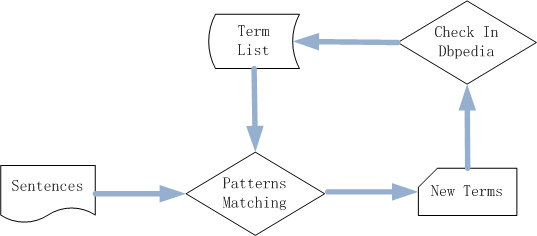
\includegraphics[scale=0.5]{images/genonto.png}
  \caption{Procedure of Finding Technical Terms}
  \label{fig:gen_onto}
\end{figure}

But not all the extracted terms can be verified in DBpedia, because some terms have multiple meanings in English, and the URLs of their DBpedia pages are unpredictable. For example, the word ``Python'' could be an animal name or a programming language.  The meaning of the programming language  has the DBpedia URL http://dbpedia.org/page/Python\_(programming\_language), which is difficult to predict. In this case, we have to check the term manually.  After getting all terms, we use Protege~\cite{noy2001creating}, an open source ontology editor, to edit the domain specific ontology, and saved it in RDF format. The interface of Protege is shown in Figure~\ref{fig:Protege}. Part of the technical ontology is shown in Figure~\ref{fig:ontology_pro}.


\begin{figure}[htbp]

  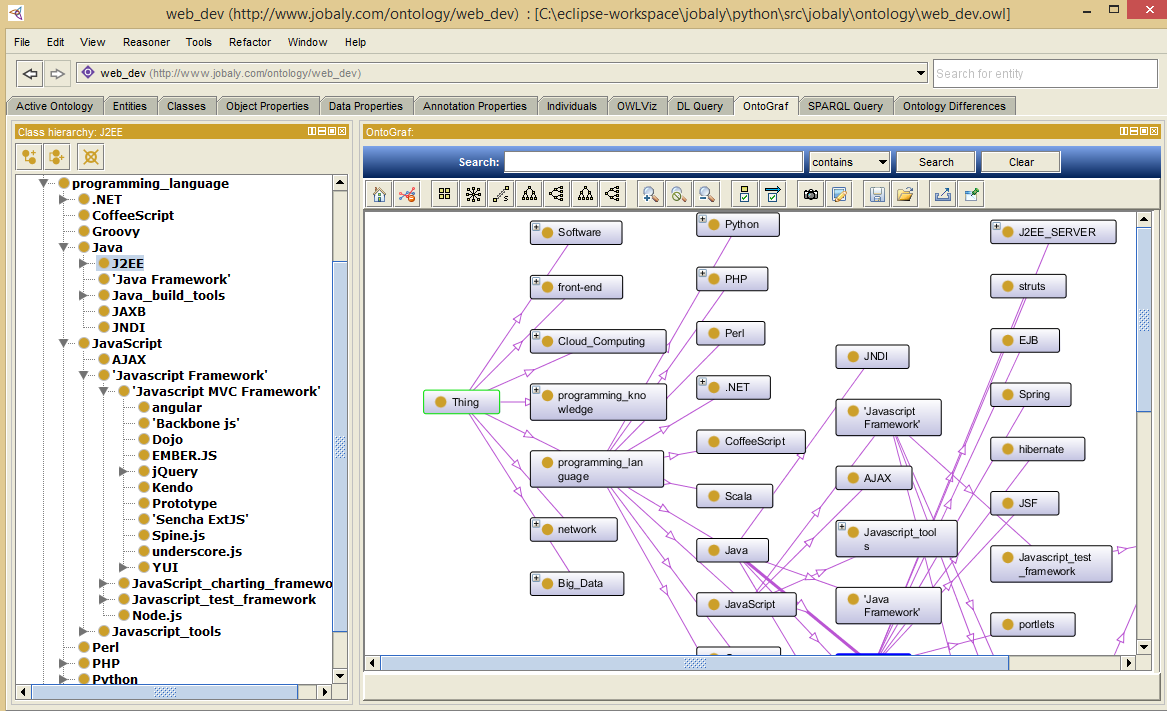
\includegraphics[scale=0.45]{images/protege.png}
  \caption{Interface of Protege}
  \label{fig:Protege}
\end{figure}

\begin{figure}[htbp]
  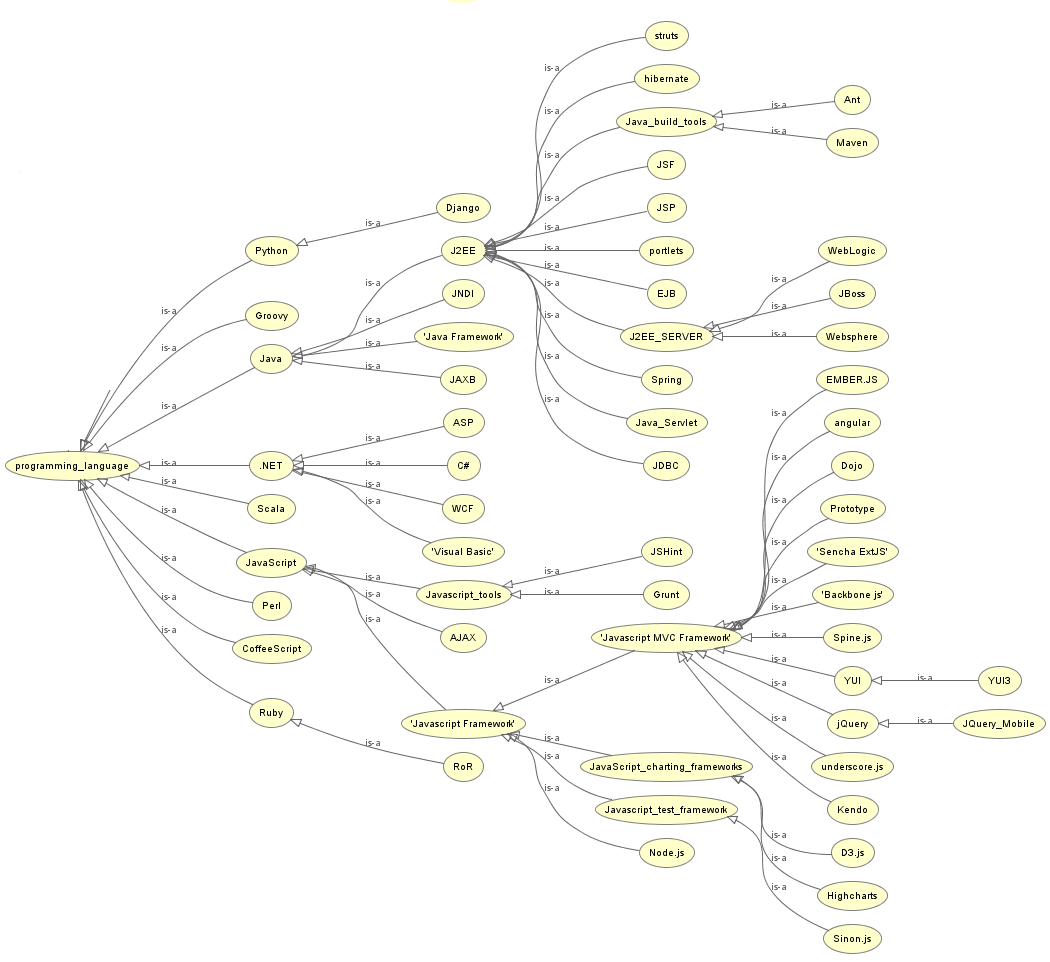
\includegraphics[scale=0.48]{images/ontology_pro.png}
  \caption{Part of Ontology}
  \label{fig:ontology_pro}
\end{figure}

\section{Ontology-Based Semantic Similarity}

S{\'a}nchez et al. \cite{sanchez2012ontology} summarized ontology-based similarity assessment into three kinds and gave both advantages and disadvantages of each approach. The three kinds of categories are: Edge-counting approaches, Feature-based measures, and Measures based on Information Content.


\subsection{Path-Based Approaches}
In path-based approaches, the ontology is viewed as a directed graph, in which the nodes are the concepts, and the edges are taxonomic relation (e.g. is-a). Rada, et al.~\cite{rada1989development} measure the similarity by the distance of two nodes in the graph. Therefore, the semantic distance of two concepts $a$ and $b$ will be:
$$ dis_{rad}(a,b) = min |path_i(a,b)| $$

Wu and Palmer~\cite{wu1994verbs} realized that the depth in the taxonomy will impact the similarity measure of two nodes, because the deeper of the nodes are in the tree, the semantic distance is smaller. Therefore they gave a new measure of ontology:
$$ sim_{w\&p}(a,b) = \frac{2 \times N_3}{N_1 + N_2 + 2 \times N_3} $$
$N_1$ and $N_2$ is the numbers of is-a links from each term to their Least Common Subsumer(LCS), $N_3$ is the number of is-a links of the LCS to the root of the ontology.

Based on the same idea, Leacock and Chodorow~\cite{leacock1998combining} also proposed a similarity measure that combined distance $Np$ between terms $a$ and $b$ and the depth $D$ of the taxonomy.
$$ sim_{l\&c}(a,b) = -\log (Np/ 2D) $$

There are some limitations of path-based approaches. First, it only considers the shortest path between concept pairs. When they meet a complex situation like multiple taxonomical inheritance, the accuracy of them will be low. Another problem of the path-based approaches is that they assume that all links in the taxonomy have uniform distance.

\subsection{Feature-Based Measures}

Feature based approaches assess the similarity between concepts as a function of their properties. They consider the degree of overlapping between sets of ontological features, like Tversky's model~\cite{tverskyfeatures}, which subtracts the non-common features from common features of two concepts.
$$  sim_{tve}(a,b) = \alpha \cdot F \left( \Psi(a) \cap   \Psi(b)  \right) - \beta  \cdot F \left( \Psi(a) \setminus   \Psi(b)  \right) - \gamma \cdot F \left( \Psi(b) \setminus   \Psi(a)  \right)  $$
Where F is salience of a set features, and $\alpha, \beta$ and $\gamma$ are weights of the contribution of each component.

Rodr{\'\i}guez and Egenhofer~\cite{rodriguez2003determining} computed similarity by summing the weighted sum of similarities between synsets, features, and neighbour concepts.
$$ sim_{re}(a,b) = w \cdot S_{synsets}(a,b) + u \cdot S_{features}(a,b) + v \cdot S_{neighborhoods}(a,b) $$

The feature-based methods consider more semantic knowledge than path-based methods. But only big ontologies/thesauri like Wordnet~\cite{miller1995wordnet} have this kind of information. Ding et al.~\cite{ding2004swoogle} revealed that domain ontologies very occasionally model any semantic feature apart from taxonomical relationship.

\subsection{Content-Based Measures}
Other approaches want to overcome the limitations of edge-counting approaches are Content-based measures. Resnik~\cite{resnik1995using} proposed a similarity measure, which depends on the amount of shared information between two terms:
$$ sim_{res}(a,b) = IC(LCS(a,b))$$
LCS is the Least Common Subsumer of terms in a ontology, and IC is Information Content, which is the negative log of its probability of occurrence, $p(a)$. Lin \cite{lin1998information} and Jiang and Conrath \cite{jiang1997semantic} extended Resnik's work. They also considered the IC of each of the evaluated terms, and they proposed that the similarity between two terms should be measured as the ratio between the amount of information needed to state their commonality and the information needed to fully describe them.
$$ sim_{lin}(a,b)=\frac{2 \times sim_{res}(a,b)}{(IC(a)+IC(b))}$$
The are also two disadvantages of the content-based measures. First, the approaches cannot compute the concepts of leave nodes, because they don't have subsumers. Second, if the concepts do not have enough common subsumers, their similarities are hard to be calculated.


\section{Statistical-Based Ontology Similarity Measure }
In this thesis, we proposed a new statistical-based ontology similarity measure. In most job descriptions, they list many skills the positions required. From observation, we found that related skills always exist in the job description simultaneously, and the positions of them are always close, e.g. HTML and CSS are always required together, and appear in the same sentence. We could see this phenomenon in Table~\ref{tab:skillinsent}, which include some skill requirement sentences from some job descriptions.

\begin{table}[ht]
\caption{Some sentences of Job Descriptions} % title of Table
\centering % used for centering table
\begin{tabular}{ | p{15cm}  | }
 \hline
    1. A high-level language such as Java, Groovy, Ruby or Python; we use Java and Groovy extensively \newline
    2. HTML5/CSS3/JavaScript, web standards, jQuery or frameworks like AngularJS would be great \newline
    3. HTML CSS and Javascript a must  \newline
    4. Experience with AJAX, XML, XSL, XSLT, CSS, JavaScript, JQuery, HTML and Web Services   \\
 \hline
\end{tabular}
\label{tab:skillinsent} % is used to refer this table in the text
\end{table}

We can see from the Table~\ref{tab:skillinsent}, the closely related concepts are always have short distance. Based on such observation, we give a new statistical-based ontology similarity measure. If two concepts $a$ and $b$ have the same direct hypernym or one  is the hypernym of the other, the similarity between them is given:
$$ S(a,b) = \frac{  N_{a \cap b} / N_{a \cup b} }{avg(\log_2( mindis(d_i,a,b) + 1 ))} $$

The numerator is the ratio of the number of documents in which the two terms exist together $(N_{a \cap b})$ and the number of documents have a least one of them $(N_{a \cup b})$. The denominator is the average $\log$ value of minimum distance $mindis(doc,a,b)$ of the two terms in documents that have them both.

We set the restriction on the position of the two concepts in the ontology, because the position of the concepts in the ontology are based on their technical similarity to others. Similar techniques will be assigned into the same category, so they should share the same hypernym, and one could be an alternative to the other. For example, we put EJB and Hibernate in the same category, because they are both J2EE persistence layer technologies, and both have the O/R mapping concept. If the applicant is familiar one of them, they can master the other very quickly. Another example is Grail and Django, they are both web frameworks and share same web design philosophies, but one of them is designed for Java web application and the other is created for Python web application. If a developer has some some experience with one of them, he/she still need to spend a lot of time to learn the other to overcome the gap between programming languages. The algorithm to calculate the similarity of two concepts is in Algorithm ~\ref{alg:alg_similarity}.

\begin{algorithm}
\caption{Calculating  Statistical-based  Similarity}
\label{alg:alg_similarity}
\KwIn{$Docs$�� $term1$, $term2$}
\KwOut{$similarity$}
$total=0$;
$hastwo=0$;
$dislist=\left [ ~~ \right ]$\;
\For{$i=1;~i~\le~len(Docs);~i++$}
{
  \If{ $ Docs_i~has~at~least~one~term $ }
    {
     $ total~+=~1 $ \;
     \If{ $ Docs_i~has~both~terms $ }
        {
           $ hastwo~+=~1 $ ;
           $ mindis~=~ minimium\_distance~(Docs_i, term1, term2) $ \;
           $ dislist.~add  ~\left(  log_2( mindis + 1 ) \right) $ \;
        }
    }
}
$ factor1~=~hastwo~ /~ total $  \;
$ factor2~=~ avg(dislist) $  \;
return $factor1 ~/~ factor2$\;
$ ~~ $
\end{algorithm}

The matrix in Table~\ref{tab:dismatrix1} show the similarity values among of some skills, which is gotten from 500 job descriptions. For example the skill HTML, the most relevant skills in order are CSS, Javascript, and jQuery,  which is the same from the perspective of experienced developers. The other example is Java, the most relevant skill in the matrix is JSP, which is also agree with the general technical knowledge.


\begin{table}

\caption{Similarities of Skills List 1}
\begin{tabular}{ c | c c c c c c  }
 \hline
  Term       &  Java  &  JDBC  & Spring & Hibernate & MySql  & Oracle   \\  \hline
  Java   &   1    & 0.0523 & 0.091  &   0.0458  & 0.0339 & 0.0608    \\  \hline
    JDBC   & 0.0523 &   1    & 0.0525 &   0.0799  & 0.006  & 0.0616   \\  \hline
   Spring  & 0.091  & 0.0525 &   1    &   0.2008  & 0.0194 & 0.0878   \\  \hline
 Hibernate & 0.0458 & 0.0799 & 0.2008 &     1     & 0.0073 & 0.115    \\  \hline
   MySql   & 0.0339 & 0.006  & 0.0194 &   0.0073  &   1    & 0.049    \\  \hline
   Oracle  & 0.0608 & 0.0616 & 0.0878 &   0.115   & 0.049  &   1      \\  \hline

\end{tabular}
\label{tab:dismatrix1}
\end{table}


\begin{table}

\caption{Similarities of Skills List 2}
\begin{tabular}{ c | c c c c c c c c }
 \hline
  Term       & Javascript & jQuery &  HTML  &  CSS   &  Java  & Python &  Ruby  &  JSP    \\  \hline
  Javascript &     1      & 0.1981 & 0.2087 & 0.2439 & 0.0665 & 0.0189 & 0.023  & 0.0253   \\
    jQuery   &   0.1981   &   1    & 0.0979 & 0.1328 & 0.0439 & 0.0142 & 0.0266 & 0.0232    \\
     HTML    &   0.2087   & 0.0979 &   1    & 0.3569 & 0.0473 & 0.0175 & 0.023  & 0.0103   \\
     CSS     &   0.2439   & 0.1328 & 0.3569 &   1    & 0.0537 & 0.0153 & 0.0181 & 0.015    \\
     Java    &   0.0665   & 0.0439 & 0.0473 & 0.0537 &   1    & 0.0498 & 0.0287 & 0.075    \\
    Python   &   0.0189   & 0.0142 & 0.0175 & 0.0153 & 0.0498 &   1    & 0.1333 & 0.0025   \\
     Ruby    &   0.023    & 0.0266 & 0.023  & 0.0181 & 0.0287 & 0.1333 &   1    & 0.012    \\
     JSP     &   0.0253   & 0.0232 & 0.0103 & 0.015  & 0.075  & 0.0025 & 0.012  &   1      \\
 \hline
\end{tabular}
\label{tab:dismatrix2}
\end{table}


\chapter{EVALUATION}

In this section, we will evaluate the performance of the key components of the system, Information Extraction and the Ontology Similarity respectively, and then the whole system.

\section{Experiments of Information Extraction }

To evaluate the performance of information extraction, we get some sentences by the sentence filters, different sentence filter can extract different kinds of sentences. We use the sentences that have degree information to explain the process:

In the experiment, we selected 100 sentences from job descriptions that are requirements of candidates degree and major. The values of degree and major are labeled manually. We use patterns to  match and extract the degree information from the sentences. The patterns are gotten from the observation of sentences. The Figure~\ref{fig:degree_accuracy} shows that when the number of  patterns increases, the accuracy of information increases as well. When we used 6 patterns, the accuracy of degree became 94\%. The accuracies of three fields matching are shown in Table \ref{tab:ieaccura}

\begin{figure}[htbp]
  \centering
  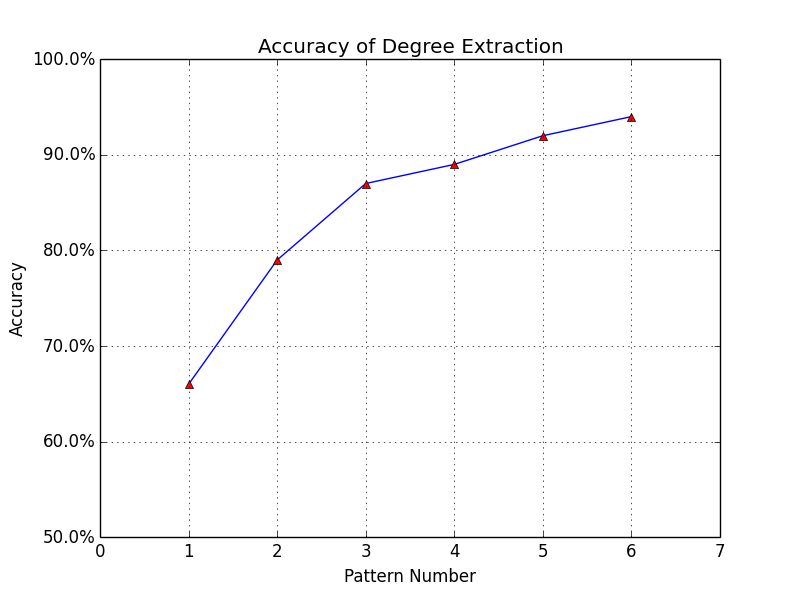
\includegraphics[scale=0.5]{images/degree_accuracy.png}
  \caption{Degree Extraction  Accuracy}
  \label{fig:degree_accuracy}
\end{figure}


\begin{table}[ht]
\caption{Information Extraction} % title of Table
\centering % used for centering table
\begin{tabular}{   | c | c | c | c |   }
 \hline
                     Field   & Pattern Num & Accuracy     \\
 \hline
                     Degree & 6         & 0.94         \\
 \hline
                     Major  & 10        & 0.85      \\
 \hline
                     Skill  & 6         & 0.82      \\
 \hline
\end{tabular}
\label{tab:ieaccura} % is used to refer this table in the text
\end{table}

\section{Experiments of Ontology Similarity}

We select some very common skills from 500 job descriptions, table~\ref{tab:dismatrix3} shows similarity values between these skills. The values in the table are the similarities between skills, the higher the value, the greater of the similarity, so the similarity between one skill and itself is 1. We select one concept, rank other concepts by their similarity value to this concept. The ranked concepts are also be given relevance scores by human judges, so we can use NDCG to evaluate the effectiveness of our approach.

\begin{table}

\caption{Skills Similarity Table 1}
\begin{tabular}{ c | c c c c c c   }
 \hline
  Term       &  Java  &  JDBC  & Spring & Hibernate & MySql  & Oracle   \\  \hline
  Java   &   1    & 0.0523 & 0.091  &   0.0458  & 0.0339 & 0.0608    \\  \hline
    JDBC   & 0.0523 &   1    & 0.0525 &   0.0799  & 0.006  & 0.0616   \\  \hline
   Spring  & 0.091  & 0.0525 &   1    &   0.2008  & 0.0194 & 0.0878   \\  \hline
 Hibernate & 0.0458 & 0.0799 & 0.2008 &     1     & 0.0073 & 0.115    \\  \hline
   MySql   & 0.0339 & 0.006  & 0.0194 &   0.0073  &   1    & 0.049    \\  \hline
   Oracle  & 0.0608 & 0.0616 & 0.0878 &   0.115   & 0.049  &   1      \\  \hline
 \hline
\end{tabular}
\label{tab:dismatrix3}
\end{table}

We use $ Normalized~Discounted~Cumulative~Gain ( NDCG )$ to evaluate the statistical-based similarity. NDCG is an important measure to evaluate the ranked retrieval results. For a set of queries $Q$, let $R(j,d)$ be the relevance score assessors gave to document $d$ for query $j$.
       $$ NDCG(Q,k) = \frac {1}{|Q|} \sum_{j=1}^{|Q|}{Z_{kj}} \sum_{m=1}^{k} \frac{2^{R(j,m)} - 1}{ \log_2(1+m)} $$

Where $Z_{kj}$ is a normalization factor calculated to make it so that a perfect ranking's NDCG at $k$ for query $j$ is 1. For queries for which $k' < k$ documents are retrieved, the last summation is done up to $k'$.

The table ~\ref{tab:simcompare1} shows how we evaluate the similarity between the concept ``Javascript'' and some other concepts. The first column is some skill names, the second column is their similarity values to Javascript, the third column is their positions ranked by the similarity values, and the fourth column is relevance value given by the judges. The NDCG value for concept Javascript is 0.94, and in table ~\ref{tab:simcompare2},  NDCG value for concept HTML is 0.97.

\begin{table}
\centering
\caption{ Javascript Similarity Evaluation : NDCG = 0.94 }
\begin{tabular}{ | c | c | c  | c |  }
 \hline
    Term     &  Similarity Value  &  Position   & Relevance     \\  \hline
    jQuery   &  0.1981            &      4      &   8        \\
     HTML    &  0.2087            &      3      &   4         \\
     CSS     &  0.2439            &      2      &   3   \\
     Java    &  0.0665            &      5      &   1   \\
    Python   &  0.0189            &      8      &   1   \\
     Ruby    &  0.023             &      7      &   1    \\
     JSP     &  0.0253            &      6      &   2    \\
 \hline
\end{tabular}
\label{tab:simcompare1}
\end{table}


\begin{table}
\centering
\caption{ HTML Similarity Evaluation : NDCG = 0.97 }
\begin{tabular}{ | c | c | c  | c |  }
 \hline
    Term      &  Similarity Value  &  Position   & Relevance     \\  \hline
  Javascript   &  0.2087           &      2      &   3        \\
     jQuery    &  0.0979           &      3      &   3         \\
     CSS     &  0.3569             &      1      &   5   \\
     Java    &  0.0473             &      4      &   1   \\
    Python   &  0.0175             &      6      &   1   \\
     Ruby    &  0.023              &      5      &   1    \\
     JSP     &  0.0103             &      7      &   3    \\
 \hline
\end{tabular}
\label{tab:simcompare2}
\end{table}


\section{Evaluation of the System}

In traditional information retrieval system, precision and NDCG are widely used measures ~\cite{manning2008introduction}. Precision ($P$) is the fraction of retrieved documents that are relevant .
       $$  Precision =  \frac{ \#(releveant~items~ retrieved)}{ \#(retrieved~items)}$$

We first used Precision@K to compare the performance our approach to some classical information retrieval models, that are Okapi BM25~\cite{robertson2009probabilistic}, Kullback-Leibler divergence, and the TF-IDF. Precision@K is the proportion of relevant documents in the first K positions and is given below:
$$ P@k = \frac{1}{k} \sum^m_{i=1} l_i 1 \left(  r(i) \leq k  \right )  $$
Where 1 is the indicator function: $1(A) = 1$ if A is true, 0 otherwise.

To evaluate job finding, we compare the results of the system with three classical information retrieval models: Kullback-Leibler divergence~\cite{zhai2008statistical},  TF-IDF~\cite{manning2008introduction} and Okapi BM25 ~\cite{robertson1995okapi}. We give the definition these measures as below. 

Kullback-Leibler divergence: the score of a document $D$ with respect to query $Q$ is given by~\cite{zhai2008statistical}:
\begin{equation}
    \begin{array}{rcl}
        s(D,Q) & = & -D( \theta_Q \parallel  \theta_D )\\
               & = &- \sum_{ \omega \in V } p (\omega \mid \theta_Q) \log \frac{ p (\omega \mid \theta_Q )}{p(\omega \mid \theta_D)} \\
               & = & \sum_{ \omega \in V } p (\omega \mid \theta_Q) \log p (\omega \mid \theta_D ) -  \sum_{ \omega \in V } p (\omega \mid \theta_Q) \log p (\omega \mid \theta_Q )  \\

    \end{array}
\end{equation}

In the equation $\theta_Q$ is language model for a query, and  $\theta_D$ is language model for a document.

TF-IDF is a Vector Space Model, which calculate Cosine Similarity between the vectors of the query $q$ and the document $d$.  $tf$ is term frequency, and $idf$ is inverse document frequency. The tf-idf weighting scheme assigns to term $t$ a weight in document $d$ given by:
$$ tf\text{-}idf_{t,d} = tf_{t,d} \times idf_{t} $$
$$ score(q,d) =  \sum_{t \in q }  tf\text{-}idf_{t,d} $$

Okapi BM25: Given a query $Q$, containing keywords $q_1, ..., q_n$, the BM25 score of a document $D$ is:

$ score(D,Q) = \sum_{ i=1 }^{n} IDF(q_i) \cdot   \frac {f(q_i,D) \cdot (k_1 + 1)}{f(q_i,D) + k_1 \cdot ( 1-b + b\cdot \frac { \left | D \right |}{avgdl})}  $

In the evaluation phrase, we created a data set of 100 job descriptions, which includes several kinds of jobs, like web developers, back-end developers, mobile developers and so on. We used 5 candidate resumes and retrieved the top 20 jobs.  The relevance value of job descriptions to each resume will be set manually. We create a query q from the resume, and treat the text of the job descriptions as documents d and apply standard ad-hoc retrieval techniques to rank the jobs.    We would like to return jobs that better match the candidates' resumes at the top. The result of Precision@k is in table~\ref{tab:job_precision}.


\begin{table}[ht]
\caption{Precision of Job Ranking } % title of Table
\centering % used for centering table
\begin{tabular}{    | c | c | c | c | c |  }
 \hline
       k     & Okapi BM25 & KL    & TF-IDF   & Ontology Similarity  \\
 \hline
       5     & 0.13       & 0.40  & 0.54     & 0.74   \\
 \hline
       10    & 0.16       & 0.36  & 0.50     & 0.66   \\
 \hline
       20    & 0.16       & 0.35  & 0.49     & 0.61   \\
 \hline

\end{tabular}
\label{tab:job_precision} % is used to refer this table in the text
\end{table}

The other measure we used is NDCG, which is explained in last section. Table ~\ref{tab:job_ndcg} shows the NDCGvalue get from different information retrieval model. The result shows that Ontology Similarity  performs the best. This agrees with results in  where it was found that finding and weighting up important concepts in long queries can improve retrieval performance.

\begin{table}[ht]
\caption{NDCG of Job Ranking } % title of Table
\centering % used for centering table
\begin{tabular}{    | c | c | c | c | c |  }
 \hline
       k    & Okapi BM25 & KL    & TF-IDF & Ontology Similarity  \\
 \hline
       5    & 0.15       & 0.34  & 0.45     & 0.78   \\
 \hline
       10   & 0.18       & 0.44  & 0.47     & 0.72   \\
 \hline
       20   & 0.19       & 0.35  & 0.45     & 0.66   \\
 \hline

\end{tabular}
\label{tab:job_ndcg} % is used to refer this table in the text
\end{table}

\section{User Study}

We evaluated the system by user studies. The purpose of the evaluation is to test the hypothesis that resume-job matching approach could return better results than keywords searching approach.

\subsection{Procedure of User Study}

At the start of the study, the experimenter introduced the system to the users. He introduced the features of the system, and gave a demo of how to the three different methods in the system to search the jobs. Then a subject was given a resume, all the resumes were download from the internet randomly. The user spent approximately 10 minutes to familiar with it, and got initial idea of what jobs are appropriate to the resume. The subject was asked to search a specific kind of job, like web developer or software engineer with the three methods. During the searching process, the time they used to search and the number of jobs they had reviewed for each method were recorded.  At the end of the study, the subject was asked to take a survey that asked  the personal judgment about the results accuracy of the three methods.


\subsection{Results}


Ten users participated user study, they are graduate and undergraduate students of Computer Science department of Texas A\&M University. The basic requirement of the users is that they can understand the meanings of technical terms of job description. The results of the study are shown in Table~\ref{tab:methodcompare}.


\begin{table}[ht]
\caption{Comparatione of Three Searching Methods } % title of Table
\centering % used for centering
\begin{tabular}{  | c | c | c | c | }
 \hline
 Method                    &  Time Used(Minutes)    & Job Reviewed & Accuracy Score  \\
 \hline
 Keyword                   & 6.3                    & 15.8         &       3.2         \\
 \hline
 Resume Matching           & 5.2                    & 14.6         &       4.1         \\
  \hline
 Keyword + Resume Matching & 4.3                    & 13.2         &       4.1       \\
  \hline
\end{tabular}
\label{tab:methodcompare} % is used to refer this table in the text\section{Pipeline of Information Extraction}
\end{table}



\chapter{CONCLUSION AND FUTURE WORK}

\section{Conclusion}
In this thesis we presented GoodJobFinder, a personalized job-r\'esum\'e matching system that can help job seekers find appropriate jobs faster and more accurately by using their r\'esum\'e contents. The key components of the system are the information extraction procedure and the ontology matching module.

In the system, job descriptions and r\'esum\'es are parsed into job models and r\'esum\'e models by the information extraction module. When searching the jobs by a r\'esum\'e, similarity values between the r\'esum\'e model and job description models are calculated in the ontology matching module. The result is sorted by the ontology similarity scores, which are the sum of similarities of different fields multiplied by their weights.
We made such contributions in our works:

\begin{enumerate}
    \item  We developed a r\'esum\'e - job matching system.
    \item  We developed a finite state transducer based matching tool to extract information from unstructured data source, which is a lightweight and flexible library, and can be extended in very easy ways.
    \item  We developed a semi-automatic approach, which can collect technical terms from hr data sources, and by which we created a domain specific ontology for recruitment.
    \item  We developed statistical-based ontology similarity measure, which can measure the similarities between technical terms .    
\end{enumerate}

In the experiment phase, we evaluated the accuracy of information extraction. We calculated the ontology similarity with the NDCG. Finally, we also tested the performance of r\'esum\'e job matching algorithm via precision@k and NDCG, which showed that our algorithm can achieve a better searching result than other information retrieval models like TF-IDF and OKpai BM25. We also compared our system with the commercial job search engine www.indeed.com, and the results showed that our system can return jobs with a better ranking.


\section{Future work}

Finding a job is a complex process, affected by both explicit and implicit factors. Our work establishes the validity of using information extraction techniques to create a more personalized job matching system, with ample potential for improvement in the future.

First we can introduce a more complex job and r��sum�� model to improve performance of the system.  In the r\'esum\'e model, we can consider hiring history and project experience of the job seekers. To improve the job description model, job responsibilities and company characteristics (size, dress code, etc.) should be considered as well.

Second, to improve searching speed of our system, we can reduce the the number of comparison by filtering out jobs that are clearly not related to r\'esum\'es. The system can classify the jobs into some different subsets, when searching jobs, the system only need to calculate the similarity between the r\'esum\'e and according subset of jobs.

GoodJobFinder is a content based recommendation system that is mostly focused on comparing the similarities between the r\'esum\'e and a relevant job description. In future work, we could introduce a hybrid recommendation system that would take advantage of other recommendation algorithms such as Collaborative Filtering. Future work on this system would place greater consideration on job seeker's personal preference like job location, career development plan, and company background.



%%%%%%%%%%%%%%%%%%%%%%%%%%%%%%%%%%%%%%%%%%%%%%%%%%%%%%%%%%%%%
\let\oldbibitem\bibitem
\renewcommand{\bibitem}{\setlength{\itemsep}{0pt}\oldbibitem}
%%%%%%%%%%%%%%%%%%%%%%%%%%%%%%%%%%%%%%%%%%%%%%%%%%%%%%%%%%%%%%%
%%%%%%%%%%%%%%%%%%%%%%%%%%%%%%%%%%%%%%%%%%%%%%%%%%%
%
%  New template code for TAMU Theses and Dissertations starting Fall 2012.
%  For more info about this template or the
%  TAMU LaTeX User's Group, see http://www.howdy.me/.
%
%  Author: Wendy Lynn Turner
%	 Version 1.0
%  Last updated 8/5/2012
%
%%%%%%%%%%%%%%%%%%%%%%%%%%%%%%%%%%%%%%%%%%%%%%%%%%%


%%%%%%%%%%%%%%%%%%%%%%%%%%%%%%%%%%%%%%%%%%%%%%%%%%%%%%%%%%%%%%%%%%%%%%
%%                           REFERENCES
%%%%%%%%%%%%%%%%%%%%%%%%%%%%%%%%%%%%%%%%%%%%%%%%%%%%%%%%%%%%%%%%%%%%%

\phantomsection
\addcontentsline{toc}{chapter}{REFERENCES}

\renewcommand{\bibname}{{\normalsize\rm REFERENCES}}

\bibliographystyle{plain}
\bibliography{jobaly}

% \include{appendices}

\end{document}
